Jets reconstructed in the ATLAS detector have their energies corrected in order to be an unbiased estimate of the particle-level jet.
This correction proceeds via multiple steps, the most significant of which include an absolute MC-based jet energy scale correction and following a correction based on auxiliary features of the jet observed in the detector.
These two steps both use numerical inversion (Chapter~\ref{ch:NI}) in order to remain independent of the underlying spectrum.
The current method of accounting for these features relies on a sequential application of numerical inversion to one feature at a time.
This Chapter introduces a new technique which can perform this correction accounting for multiple feature simultaneously, accomplished through the use of neural networks.
The multivariate nature of the new technique allows to account for correlations between the energy dependence on multiple features, which is not accounted for in the current method.
The new technique, called \textit{generalized numerical inversion}, generalizes numerical inversion by retaining the key property of being independent of the underlying prior distribution, while accounting for multiple features simultaneously.
This new technique further improves the correction on a variety of metrics relative to the sequential method.
As a method for improving the jet energy scale and resolution, the new technique is widely applicable to analyses in ATLAS, and in particular to the two searches presented in this Thesis (Chapter~\ref{ch:HBSM} and Chapter~\ref{ch:CWoLa}).
The results presented in this Chapter are published in~\cite{ATL-PHYS-PUB-2018-013}.

\section{Introduction}
\label{sec:GenNI:intro}
%-------------------------------------------------------------------------------
%Jets are collimated sprays of particles resulting from the fragmentation of high energy quarks and gluons.
The two searches presented in this Thesis (Chapter~\ref{ch:HBSM} and Chapter~\ref{ch:CWoLa}) use jets extensively, and besides that nearly every analysis at the Large Hadron Collider (LHC) uses jets in some capacity, both Standard Model (SM) measurements and searches for physics beyond the SM.
All of these analyses rely on an accurate and precise measurement of the jet energy.
As mentioned in Section~\ref{sec:ATLAS:jet_calibration}, due to various distortions arising from detector effects, the reconstructed jet energy deviates from the particle-level jet energy in the absence of a detector.
These distortions are corrected for using a series of calibration steps~\cite{PERF-2016-04,Aad:2011he,Schwartzman:2015ada}.
All of these steps proceed ultimately via numerical inversion, the properties of which are expounded upon in detail in Chapter~\ref{ch:NI}.
This Chapter is concerned with improving one particular and important part of the current calibration procedure, the Global Sequential Calibration (GSC).
This step incorporates auxiliary measurements about the jet, such as its reconstructed charged particle multiplicity, to improve the overall quality of the energy reconstruction~\cite{ATLAS-CONF-2015-002}.

The correction based on auxiliary features intends to further improve the jet calibration via a few metrics.
First, using features correlated with the provenance of the jet, the difference in energy scale between, e.g., quark and gluon jets can be reduced.
Second, by reducing the dependence of the scale on auxiliary features, the effects of mismodeling in the underlying spectrum of these features can be mitigated.
Third, the correction can remove the additional component of the jet energy resolution relative to the particle-level quantity due to the spread of these underlying features.

The current method for the GSC treats the impact of each auxiliary feature sequentially and independently, which requires the set of features used in the correction to be chosen in such a way to have uncorrelated effects on the jet energy.
However, there is additional information available which could improve the calibration and yet is not used in the current GSC because of this requirement of uncorrelation.
This Chapter presents a new technique using neural networks to simultaneously take into account multiple auxiliary variables in this correction which may or may not have correlated effects on the jet energy.
The technique relies both on the general capacity of neural networks to approximate well complicated functions in high dimensions~\cite{HORNIK1991251} and on recent advances in jet substructure~\cite{Larkoski:2017jix} which indicate useful features for applying this correction.
As mentioned in Chapter~\ref{ch:NI}, it is important that the calibration is independent of the underlying \pt{} spectrum, and therefore that ultimately it relies on numerical inversion.
The new technique presented here, called \textit{generalized numerical inversion}, incorporates neural networks into the numerical inversion framework in order to accomplish both goals of simultaneously taking into account the effect of multiple auxiliary variables and of remaining independent of the underlying spectrum.
Ultimately this technique is shown to improve the overall quality of the jet calibration on the three metrics outlined above.

This Chapter is organized as follows.
Section~\ref{sec:GenNI:atlas} discusses the simulated samples used in this study and Section~\ref{sec:GenNI:jetreco} briefly reviews the GSC and describes it in the notation used in this Thesis.
Generalized numerical inversion is described in Section~\ref{sec:GenNI:genni} and first results using this new method are presented in Section~\ref{sec:GenNI:results}.
There is a discussion of the results in Section~\ref{sec:GenNI:discussion} and the Chapter concludes with Section~\ref{sec:GenNI:conclusion}.

%-------------------------------------------------------------------------------
%\section{ATLAS Detector and Event Simulations}
\section{Event Simulations}
\label{sec:GenNI:atlas}
%-------------------------------------------------------------------------------

Studies documented within this chapter are performed using a variety of Monte Carlo (MC) simulated samples (Section~\ref{sec:ATLAS:simulation}).
Dijet events are generated at Leading Order (LO) in \PYTHIA 8.1~\cite{Sjostrand:2007gs} with the $2 \rightarrow 2$ matrix element convolved with the NNPDF2.3LO Parton Distribution Function (PDF) set~\cite{Ball:2012cx} and using the A14 set of tuned parameters~\cite{ATL-PHYS-PUB-2014-021}.
An additional sample is simulated using \textsc{Herwig} 7.0~\cite{Bellm:2015jjp} using the NNPDF3.0 NLO PDF and the default set of tuned parameters for the underlying event.
Both \PYTHIA{} and \textsc{Herwig} are interfaced with \textsc{EvtGen} for heavy flavor decays~\cite{Lange:2001uf,ATL-PHYS-PUB-2014-008}.

%Additional dijet events are simulated using different generators, in order to study the impact of modeling uncertainties. \SHERPA 2.1~\cite{Gleisberg:2008ta} generates events using multi-leg $2\rightarrow N$ matrix elements, which are matched to parton showers following the CKKW prescription~\cite{Catani:2001cc}. These \SHERPA events are simulated using the CT10 PDF set~\cite{Lai:2010vv} and default \SHERPA event tune. \HERWIGpp 2.7~\cite{Bahr:2008pv,Corcella:2000bw} provides a sample of events where additional radiation is showered using angular-ordering. These events are generated with the $2\rightarrow 2$ matrix element, convolved with the CTEQ6L1PDF set~\cite{Pumplin:2002vw} and configured with the UE-EE-5 tune~\cite{Gieseke:2012ft}.

%mc16_13TeV.364446.Herwig7EvtGen_H7UE_NNPDF30nlo_jetjet_JZ3.deriv.DAOD_STDM9.e5989_s3126_r9364_r9315_p3306)

All simulated events have been reconstructed using a full simulation of the ATLAS detector~\cite{SOFT-2010-01} implemented in \GEANT 4~\cite{Agostinelli:2002hh}, which describes the interactions of particles with the detector and the subsequent digitization of analog signals.
The effects of multiple simultaneous $pp$ collisions (pile-up) are simulated with minimum bias $pp$ collisions using \PYTHIA 8.1 and overlaid on the nominal dijet interactions.

%-------------------------------------------------------------------------------
\section{Global Sequential Calibration}
\label{sec:GenNI:jetreco}
%-------------------------------------------------------------------------------
As mentioned in Section~\ref{sec:ATLAS:jet_calibration}, the ATLAS jet calibration proceeds via multiple steps.
The largest correction is the absolute MC-based correction which brings the overall scale of the reconstructed jet $E$ to the truth or particle-level $E$.
The step immediately proceeding is the GSC, which corrects the dependence of the jet \pt{} on various jet quantities derived from information in the tracker, calorimeter, and muon system~\cite{PERF-2011-04,Aaboud:2019ibw,PERF-2016-04}.

%The goal of this correction is to make the response more similar between quark- and gluon-initiated jets, and furthermore reduces the uncertainty due to jet fragmentation modeling for a given jet type.

%The focus of this Chapter is on improving the method used for the MC-based residual calibration of the jet $p_\text{T}$ on various jet quantities following an inclusive calibration, which in ATLAS is accomplished with the GSC.

%To perform a calibration in $\pt$, one may want to learn a function that predicts $\pttrue$ given $ \ptreco$.
%While straightforward, this method depends on the distribution of $p_\text{T}^\text{true}$ and thus renders the calibration dependent on the event sample from which it is derived.
%Moreover, this method does not guarantee that $f(x) \approx x$ even for the sample used to derive the calibration.
%After applying the learned function it should be the case that $p_\text{T}^\text{reco}\approx \langle p_\text{T}^\text{true}|p_\text{T}^\text{reco} \rangle$, but $f(x) = \langle p_\text{T}^\text{reco}|p_\text{T}^\text{true}=x\rangle\approx x$ may not necessarily be satisfied.
%%In particular, it may be the case that $f(x)\approx x$ for the sample used for deriving the calibration, but $f(x)\neq x$ (non-closure) for other samples. %Impossible...if f(x)=x for one sample then it's true for all samples, that's the point.
%A potential modification of the naive procedure is to enforce that the distribution of $p_\text{T}^\text{true}$ used in the learning is uniform over a particular range.
%However, one can show that if $f(x)$ is nonlinear or if the resolution $\sigma( p_\text{T}^\text{reco}|p_\text{T}^\text{true})$ is nonconstant, then even with this modification there can be large non-closures.
%Since both of these properties are true of jet reconstruction in ATLAS, this simple fix does not solve the non-closure problem.
%
%An approach that can be used to ensure that the calibration is independent of the $p_\text{T}^\text{true}$ distribution is called numerical inversion, which is the method used in ATLAS for the jet energy corrections.  Instead of learning to predict
%%\footnote{As stated above, the inclusive calibration actually corrects the jet energy; for simplicity and because the focus of this chapter is about improving the GSC that corrects the $p_\text{T}$, only the transverse momentum is mentioned here.} 
%$p_\text{T}^\text{true}$ given $p_\text{T}^\text{reco}$, numerical inversion does exactly the opposite - by using $f(x)$ directly, $p_\text{T}^\text{reco}$ is calibrated via $p_\text{T}^\text{reco}\mapsto \ptrecohat \equiv f^{-1}(p_\text{T}^\text{reco})$.  This procedure is inherently independent of the distribution of $p_\text{T}^\text{true}$ and under a wide variety of circumstances~\cite{Cukierman:2016dkb}, the response closes ($\hat{R}(x)\equiv\langle \ptrecohat/\pttrue|p_\text{T}^\text{true}=x\rangle\approx 1$) following the calibration.  

There may be a little confusion here in moving from the calibration of \Et{} to \pt{}.
The first thing to note is that this is just simply how the ATLAS calibration does it, first an absolute correction to \Et{} and then following a residual correction to \pt{}.
The second thing to note is that \Et{} and \pt{} have a well-defined relation: $\Et=\sqrt{\pt^2+m^2}$, where $m$ is the mass of the jet.
The GSC is only applied to small-$R$ jets, intended to apply to quark- and gluon-initiated jets in which the true mass is either $0$ or much less than the \pt{} (the lowest \pt{} in the calibration is 20 \GeV, while the highest quark mass reconstructed in a small-$R$ jet is the bottom quark, with mass of $\sim4$ \GeV).
This is related to the fact that the opening angle of a jet is generically roughly $\Delta R \sim \frac{2m}{\pt}$~\cite{Shelton:2013an}; for a small-$R$ jet, with $\Delta R$ parameter of 0.4, $\frac{m}{\pt}<0.2$.
Because of the negligibility of this term, for small-$R$ jets it is the case that $\Et\sim\pT$, and the term ``jet energy'' correction is used somewhat loosely in this Chapter (and in the previous one) to refer to the ATLAS jet \Et{} and \pT{} corrections in the calibration.
Generally the distinction is not important, but where it is the text is clear about what is being corrected.

For large-$R$ jets, the $\Delta R$ parameter is $1.0$, allowing for jets with larger ratios of $\frac{m}{\pt}$.
The GSC is not applied to these jets, but rather after the inclusive \Et{} correction an energy-dependent mass calibration is applied (Section~\ref{sec:ATLAS:jet_calibration}).
The Author has contributed to work which directly uses the techniques developed in this Chapter to employ neural networks to simultaneously calibrate the mass and energy of large-$R$ jets~\cite{ATL-PHYS-PUB-2020-001}.

As mentioned in Chapter~\ref{ch:NI}, after the inclusive correction it is approximately true that $f(x)\equiv \langle p_\text{T}^\text{reco}|p_\text{T}^\text{true}=x\rangle = x$\footnote{In practice $f(x)$ is measured using the mode of the distribution rather than the mean.} (Equation~\ref{eqn:NI:closure_mode_text}), i.e. that the calibration closes and that the average reconstructed or detector-level jet \pt{} ($p_\text{T}^\text{reco}$) is an unbiased estimator\footnote{An estimate $\hat{\theta}$ of a fixed but unknown parameter $\theta$ is an unbiased estimator if, for all values of $\theta$, $\mathbb{E}\left[\hat{\theta}|\theta\right] = \theta$.} of the truth or particle-level \pt{} ($p_\text{T}^\text{true}$)
\footnote{Of course, this statement is subject to the stipulations mentioned in that Chapter, and in fact a major result from that study was understanding exactly how and why the calibration \textit{does not} close. However, ultimately the understanding from that study was that the major non-closures would be a bigger issue at higher pile-up conditions that will exist at the LHC in the future.}.
The reason to follow this with the GSC is that even though the overall response closes, $f(x)$ may have a residual dependence on auxiliary information available from the detector.

The GSC uses $5$ auxiliary features which can be grouped into $3$ categories based on the effect being corrected for.
The first two features are the number of tracks in the jet (associated via ghost association~\cite{Cacciari:2008gn}) and the width of tracks in the jet (the average \pt-weighted distance of tracks from the jet axis).
Since the calorimeter-cell response is non-linear due to noise suppression, a jet with more particles (and therefore softer on average for fixed total \pt{}) will tend to have a lower measured energy than a jet with a few hard particles.
The number of tracks in the jet is a good but not perfect measure of the number of particles, as tracks are insensitive to pile-up, but only correspond only to charged particles.
This effect is correlated to the provenance of the jet, as gluon jets tend to have more particles and a wider radiation pattern than quark jets~\cite{Salam:2009jx}.
The track width is used to further discriminate between gluon and quark jets, and therefore gain more information about the number of particles produced in the jet.
The correction for the first two features has the benefit of making the response more similar between quark- and gluon-initiated jets, which reduces the sample dependence of the jet \pt{} closure.

The second two features are the fraction of jet energy in the final layer of the electromagnetic calorimeter and in the first layer of the hadronic calorimeters; these features account for energy loss in the dead material between the electromagnetic and hadronic calorimeters.

The final feature counts the number of muon segments behind the jet that register hits; this feature accounts for energy not measured in the calorimeter due to showers that punch through to the MS.

%The goal of the GSC is to correct the jet \pt{} for each of these effects.
%In doing so, the GSC improves the jet \pt{} closure in all regions of the parameter space, reduces the uncertainty due to jet fragmentation modeling, and reduces the spread of the jet \pt{} inclusively.

Let $\theta$ represent the available auxiliary information about a jet\footnote{Note that $\theta$ can be a single value or a vector with multiple features.}, e.g. the $5$ features used in the GSC.
Then, the function $f$ can be generalized as $f_\theta(x)\equiv \langle p_\text{T}^\text{reco}|p_\text{T}^\text{true}=x,\theta\rangle$.

%Although it may seem intuitive that one would want to correct for the dependence of the jet energy on auxiliary variables if such a dependence exists, it is worth delving into exactly what the reasons and implications of such a correction are.

In general, if it is found that the jet energy $f_\theta(x)$ depends on some auxiliary variable $\theta$, then it is desirable that the calibration removes this dependence, for a few reasons.
First, if the distribution of $\theta$ is sample-dependent, e.g. correlated with the jet originating parton, then there could be closure in one sample but not another, which could cause nonoptimal selections in the final analysis cuts.
Second, if $\theta$ is not well-modeled by the simulation then even though there may be closure in the simulation there may not be closure in the data, and this could introduce systematic uncertainties in the final calibration.
Third, there is a degradation of the resolution $\sigma(x)$ due to the spread of $\theta$, which can cause the sensitivity of the final analysis selection to be worse than with an undegraded resolution.
These are the three metrics by which we judge the performance of the GSC and of generalized numerical inversion in this Chapter.

However, this third point is more subtle than it naively appears.
While it is true that there is a degradation of the resolution due to the spread of $\theta$, it is \emph{not} the case that the resolution always gets better when the dependence of the response on an auxiliary variable is corrected.
In particular, there exist certain situations where correcting for the dependence of the response on an auxiliary variable can actually make the resolution worse.
This can occur, for example, if $\theta$ is correlated with $\pttrue$ in such a way that removing the correlation between $\ptreco$ and $\theta$ also removes some of the correlation between $\ptreco$ and $\pttrue$.
These situations are explored in more detail in Appendix~\ref{sec:GenNI_app:auxiliary}.

It is important to note that this auxiliary information $\theta$ is available at the detector or reconstructed level.
Therefore, while $f_\theta(x)$ is derived in simulation, for a given jet at detector level $\theta$ is known and $f_\theta(x)$ can be inverted as usual across its argument to give the calibration function.
For $\theta\in\mathbb{R}$, the correction is therefore given by $p_\text{T}^\text{reco}\mapsto \ptrecohat = f_\theta^{-1}(p_\text{T}^\text{reco})$.
In practice, the distribution of $\theta$ is binned and the numerical inversion is performed for different functions in each bin of $\theta$.


When $\theta\in\mathbb{R}^n$, a sequential calibration like the GSC (for which $n=5$) proceeds with a sequential (as the name suggests) application of numerical inversion:

\begin{align}
\label{eqn:GenNI:gsc}
p_\text{T}^\text{reco}\mapsto \ptrecohat = f_{\theta_{n}}^{-1}\left(\cdots f_{\theta_{2}}^{-1}\left(f_{\theta_{1}}^{-1}\left(p_\text{T}^\text{reco}\right)\right)\cdots\right).
\end{align}

%Note that Eq.~\ref{eq:gsc} assumes that $f_{\theta_{i}}(x)$ is independent of $\theta_{j\neq i}$; otherwise, there will be a residual dependence on $\theta_i$ after the sequential calibration is applied.
The sequential method removes all residual dependencies when $f_{\theta_{i}}(x)$ is independent of $\theta_{j\neq i}$, i.e. when $f_{\theta}(x)$ is entirely determined by one feature at time.
If there are such dependencies of $f_{\theta}(x)$ on more than one feature $\theta_i$, then there could be residual dependencies on some combination of the $\theta_i$ after the full sequential correction.

%-------------------------------------------------------------------------------
\section{Generalized Numerical Inversion}
\label{sec:GenNI:genni}
%-------------------------------------------------------------------------------

The idea of generalized numerical inversion is to simply replace the sequential approach in Equation~\ref{eqn:GenNI:gsc} with a single inversion: $p_\text{T}^\text{reco}\mapsto \ptrecohat = f_{\theta_1,...,\theta_n}^{-1}(p_\text{T}^\text{reco})$.  Binning the response in $n$ dimensions would require significant computing resources and so is practically infeasible.  An unbinned approach that can simultaneously capture the dependence on many features is needed to exploit the potential correlations in the response on the $\theta_i$.  One powerful tool for this purpose is a neural network.  In principle, neural networks can approximate any smooth function~\cite{Cybenko1989,HORNIK1991251} and have been shown to provide excellent performance for a wide variety of classification and regression tasks with limited training data.  Inverting a neural network can be non-trivial, so the procedure for generalized numerical inversion is adapted as follows:

\begin{enumerate}
  \item Learn a neural network approximation $L(x,\theta)$ to the function $f_\theta(x)=\langle p_\text{T}^\text{reco}|p_\text{T}^\text{true}=x,\theta\rangle$.  \\ Note that, if $\theta$ is a vector with $n$ features, then $L(x,\theta):\mathbb{R}^{n+1}\rightarrow\mathbb{R}$.
\item Learn a neural network $C(L(x,\theta),\theta)$ that tries to predict $x$ given $\theta$ and $L(x,\theta)$.  This is an approximation to the family of functions $f^{-1}_\theta(x)$.  Note that learning the inverse this way is technically simple since $L$ is single-valued.
\item Calibrate with $\ptreco \mapsto \ptrecohat = C(\ptreco,\theta)$.  The calibration non-closure is defined as usual as the deviation of $\langle \ptrecohat/\pttrue | \pttrue=x,\theta\rangle$ from $1$.
\end{enumerate}

There are therefore two learning stages in this procedure.
The first step learns a neural network that predicts the average behavior of $p_\text{T}^\text{reco}$ given $p_\text{T}^\text{true}$ and $\theta$ while the second network tries to approximate a single-valued function.
In principle, the above procedure could be applied to the entire jet calibration procedure described in Section~\ref{sec:ATLAS:jet_calibration}, but the focus here is on the component addressing residual dependencies, following the inclusive jet energy calibration.

A schematic of the generalized numerical inversion method is shown in Figure~\ref{fig:GenNI:schematic}.
\begin{figure}[h!]
  \centering 
  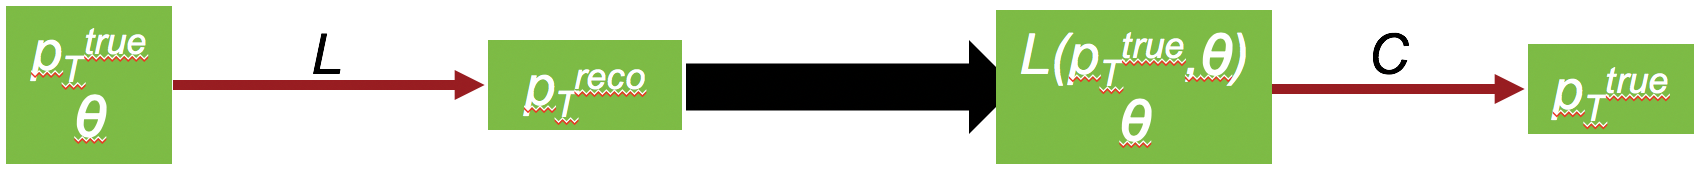
\includegraphics[width=0.9\textwidth]{{figures/GenNI_schematic.png}}
  \caption{
    A schematic of the generalized numerical inversion method.
    First, a neural network  $L$ is trained to learn $\ptreco$ from $\pttrue$ and $\theta$, which is an approximation to the functions $f_\theta(x)$.
    Then, a second neural network $C$ is traind to learn $\pttrue$ from $L(\pttrue,\theta)$ and $\theta$, which is an approximation to the functions $f^{-1}_\theta(x)$.
    Finally, $C$ is used as the calibration function.
    }
  \label{fig:GenNI:schematic}
\end{figure}

\FloatBarrier

%-------------------------------------------------------------------------------
\section{Results}
\label{sec:GenNI:results}
%-------------------------------------------------------------------------------

To illustrate the potential of generalized numerical inversion, an example is provided using jets from the ATLAS full detector simulation.
Neural network training is performed using scikit-learn~\cite{scikit-learn} with a simple two-layer feed-forward neural network that has 100 hidden nodes in each layer and a rectified linear unit activation function.
To lay the groundwork for application to the full GSC, two key jet features are studied: the number of tracks above 1 GeV associated to the jet ($n_\text{track}$) and the average track radius\footnote{The GSC currently used in ATLAS uses instead the track width, which is the average track radius multiplied by $(n_\text{track}+1)$.  The residual dependence of the $n_\text{track}$-calibrated response on the track width is negligible and is thus not useful for benchmarking generalized numerical inversion as the sequential calibration is nearly the same as the simultaneous calibration. 
  %There are observables which blah.
}:
\[
\Rtrack \equiv
\begin{cases}
  \frac{1}{n_\text{track}+1}\sum_\text{tracks}(p_\text{T,track}/\sum_\text{tracks'} p_\text{T,track'})\times \Delta R_\text{track,jet} & \text{if $\ntrack>0$}\\
  -1 & \text{if $\ntrack=0$}
\end{cases}
\]
The average track radius is also sometimes denoted more explicitly as $\langle p_\text{T,frac}\times \Delta R \rangle$.
As mentioned in Section~\ref{sec:GenNI:jetreco}, these observables account are correlated with the type of parton that produced the jet (gluon or quark), and account for effects on the $\pt$ response due to the non-linear calorimeter-cell response.
%Since gluon jets tend to have more particles and have a wider radiation pattern than quark jets, these observables are also correlated with the type of parton that produced the jet, and therefore there is a difference in response between quark and gluon jets.
%The entire effect is not accounted for, as the tracker is only sensitive to charged particles; however, associated tracks are used as they are insensitive to pile-up and provide a good measure of these jet radiation properties.
The underlying distributions of these two variables are given in Figure~\ref{fig:GenNI:distributions}.
\begin{figure}[h!]
  \centering 
  \subfloat[]{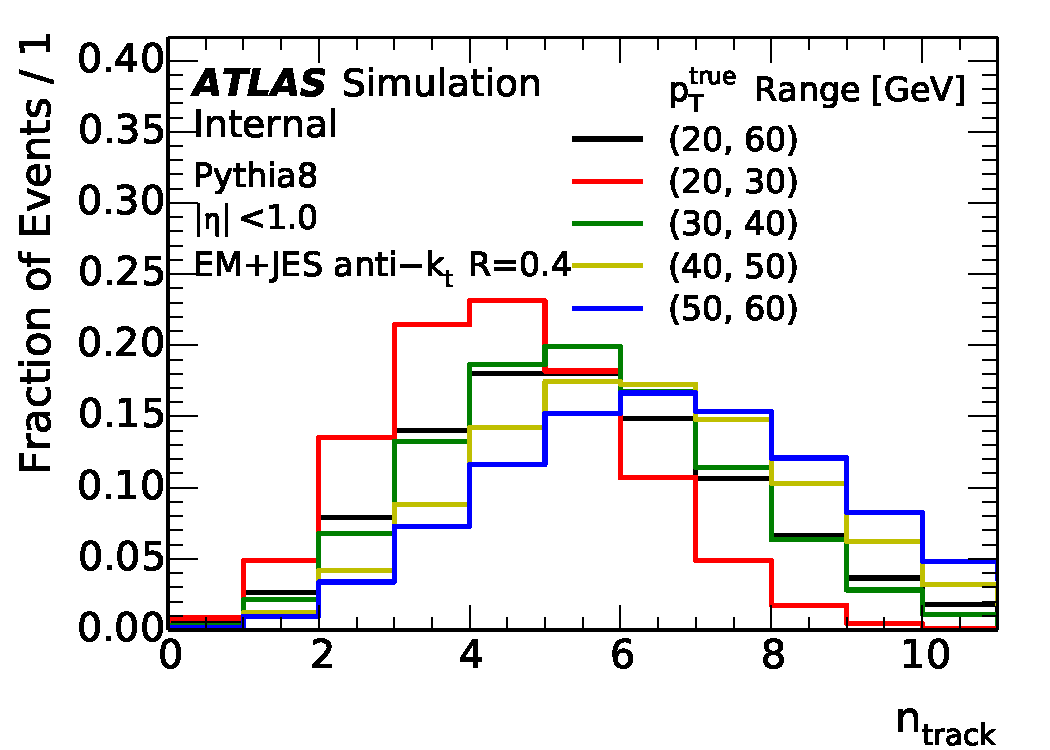
\includegraphics[width=0.45\textwidth]{{figures/hist_nTrack_shape_.pdf}}}
  \subfloat[]{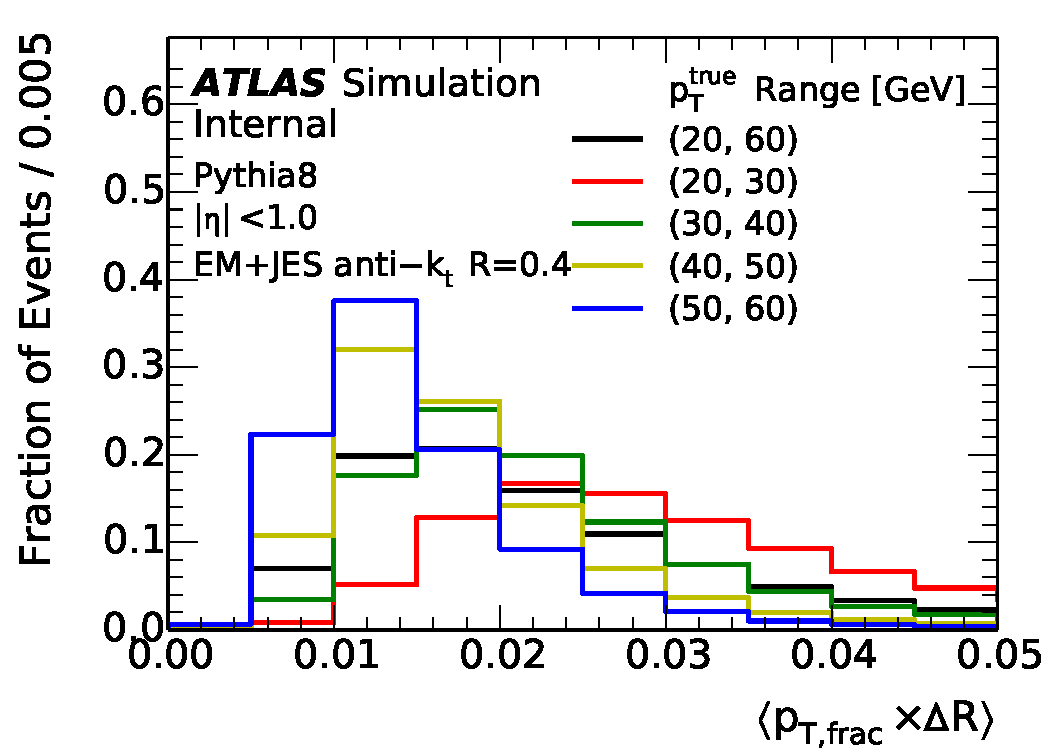
\includegraphics[width=0.45\textwidth]{{figures/hist_wTrack_mod_shape_.pdf}}}
  \caption{
    The distributions of (a) $n_{\text{track}}$ and (b) $\Rtrack=\langle p_\text{T,frac}\times \Delta R \rangle$ in bins of $\pttrue$.
    }
  \label{fig:GenNI:distributions}
\end{figure}

Figure~\ref{fig:GenNI:R_scan} shows the dependence of the response (following the inclusive energy calibration) on $n_\text{track}$ and $\Rtrack$.
The response depends strongly on these two quantities, varying by about 10-20\% across the accessible range.
The trends are also not uniform in jet $p_\text{T}$ - the response of lower $p_\text{T}$ jets shows a stronger dependence on both $n_\text{track}$ and $\Rtrack$.
%While the dependence of the response on $\Rtrack$ is non-linear, the residual dependence as shown in Fig.~\ref{fig:GenNI:R_scan}(a) is approximately linear and so is well-characterized by $dR/dn_\text{track}$.  

%Should describe the NN setup here before presenting results.  Figure~\ref{fig:GenNI:R_scan} shows the dependence of $f(x)$ on $n_\text{track}$ in several bins of true jet $p_\text{T}$.  Continue to describe the results from \href{https://indico.cern.ch/event/718661/contributions/2960406/attachments/1629909/2597628/GenNI_4.10.18.pdf}{This recent JES/JER talk}.


In order to understand the performance provided by a simultaneous instead of a sequential approach, approximations are derived for the calibration functions $f_{\text{n}_\text{track}}(x)$, $f_{\Rtrack}(x)$, and $f_{\text{n}_\text{track},\Rtrack}(x)$, and the sequential calibration $f^{-1}_{\Rtrack}(f^{-1}_{\text{n}_\text{track}}(p_\text{T}^\text{reco}))$ is compared with the simultaneous calibration $f^{-1}_{\text{n}_\text{track},\Rtrack}(p_\text{T}^\text{reco})$.
The sequential calibration presented here differs in some details with the standard GSC used in ATLAS; a major difference is that the calibration presented here does an unbinned fit to $\ptreco$ and the feature $\theta$ while the GSC does a binned fit which is then smoothed.
To control for this ability of the neural network to operate unbinned, the generalized numerical inversion approach is used for both the one- and two-feature cases in order to study only the differences between the sequential and the simultaneous calibrations.  
However, importantly the sequential approach demonstrated here does no worse than the GSC in correcting for the residual dependence of the response.

%The learned functions in the sequential calibration, $L(\pttrue,\text{n}_\text{track})/\pttrue$ and $L(\pttrue,\Rtrack)/\pttrue$, are presented in Figure~\ref{fig:GenNI:ntrack_wtrackmod_seq_LR_CR_scan}(a) and (d).
The learned functions $L$ in the sequential calibration are presented in Figures~\ref{fig:GenNI:ntrack_wtrackmod_seq_LR_CR_scan:a} and~\ref{fig:GenNI:ntrack_wtrackmod_seq_LR_CR_scan:d}.
As expected, Figure~\ref{fig:GenNI:ntrack_wtrackmod_seq_LR_CR_scan:a} looks similar to Figure~\ref{fig:GenNI:R_scan:a}, as the neural network has learned to approximate the shape of the response with respect to $\ntrack$ (Figure~\ref{fig:GenNI:ntrack_wtrackmod_seq_LR_CR_scan:d} is not expected to look similar to Figure~\ref{fig:GenNI:R_scan:b}, since the previously applied $\ntrack$ correction affects the dependence of the response on $\Rtrack$).
The ratio of $\ptreco$ to $L(\pttrue)$ (for the appropriate $\theta$, at the appropriate step of the sequential calibration) is shown in Figures~\ref{fig:GenNI:ntrack_wtrackmod_seq_LR_CR_scan:b} and ~\ref{fig:GenNI:ntrack_wtrackmod_seq_LR_CR_scan:d}, and the ratio is very close to $1$, indicating the learning step is working properly.
The closure of the calibrations at each step of the sequence is shown in Figures~\ref{fig:GenNI:ntrack_wtrackmod_seq_LR_CR_scan:c} and~\ref{fig:GenNI:ntrack_wtrackmod_seq_LR_CR_scan:f}.
In both cases, the calibration closes, with an average calibrated response at unity, independent of the features.

\begin{figure}[h!]
  \centering 
  \subfloat[]{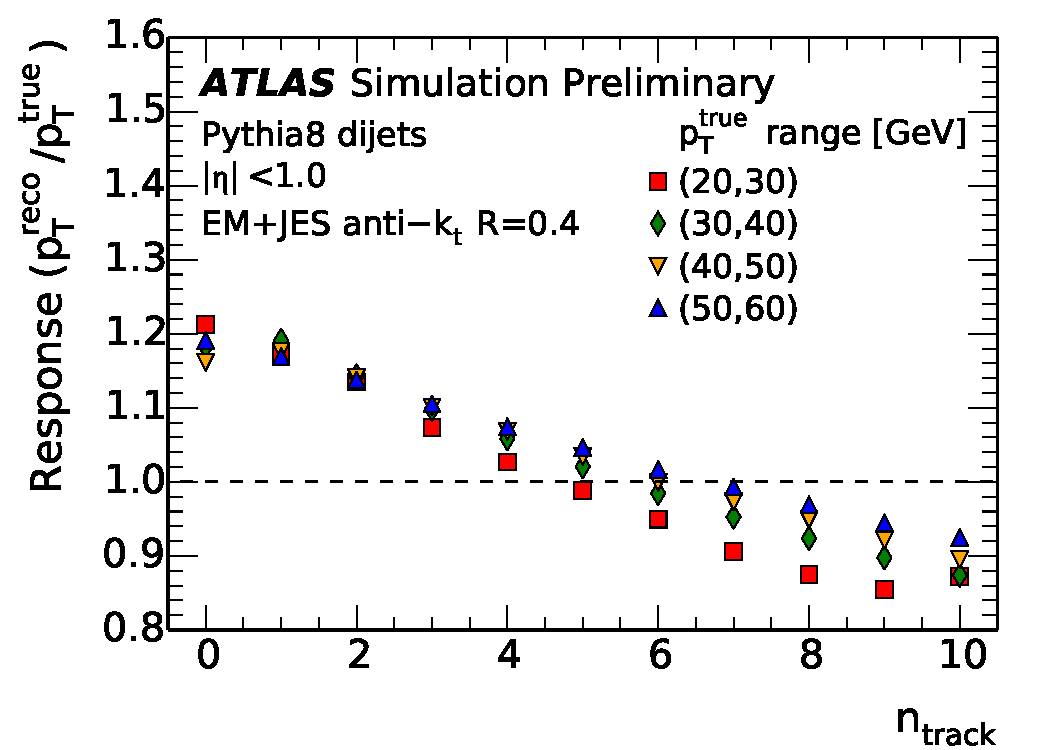
\includegraphics[width=0.45\textwidth]{{figures/R_nTrack_scan_preliminary.pdf}}\label{fig:GenNI:R_scan:a}}
  \subfloat[]{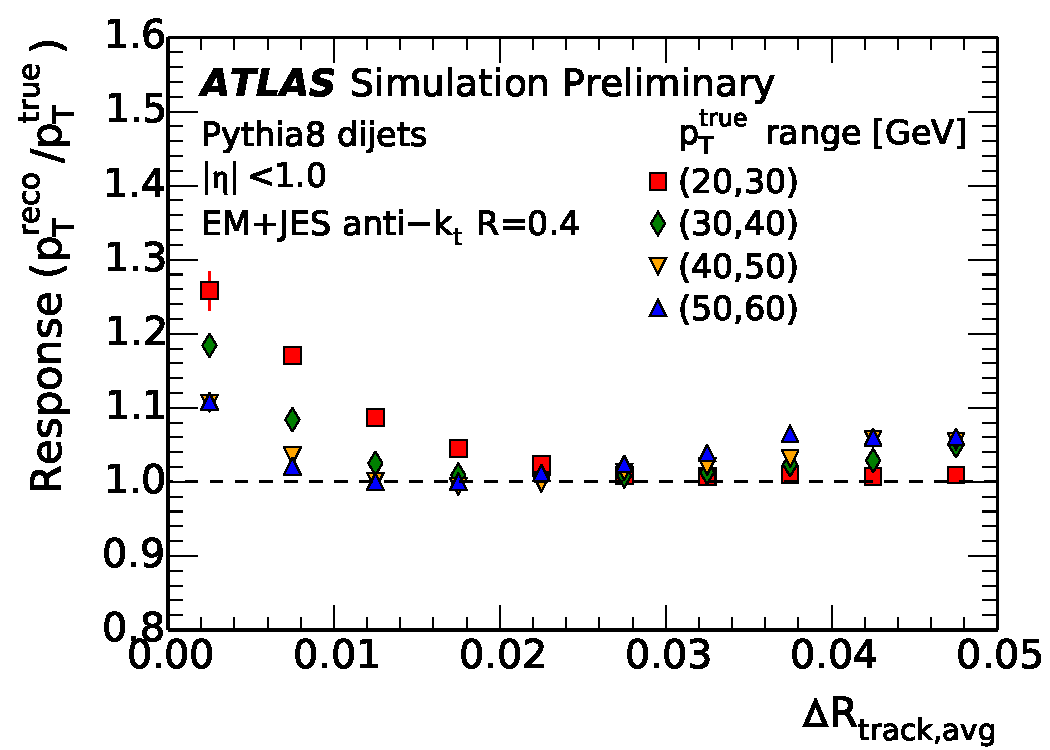
\includegraphics[width=0.45\textwidth]{{figures/R_wTrack_mod_scan_preliminary.pdf}}\label{fig:GenNI:R_scan:b}}
  \caption{The dependence of the response on (a) $n_\text{track}$ and (b) $\Rtrack$ in several bins of truth jet $p_\text{T}$.
    }
  \label{fig:GenNI:R_scan}
\end{figure}


\begin{figure}[h!]
  \centering 
  \subfloat[]{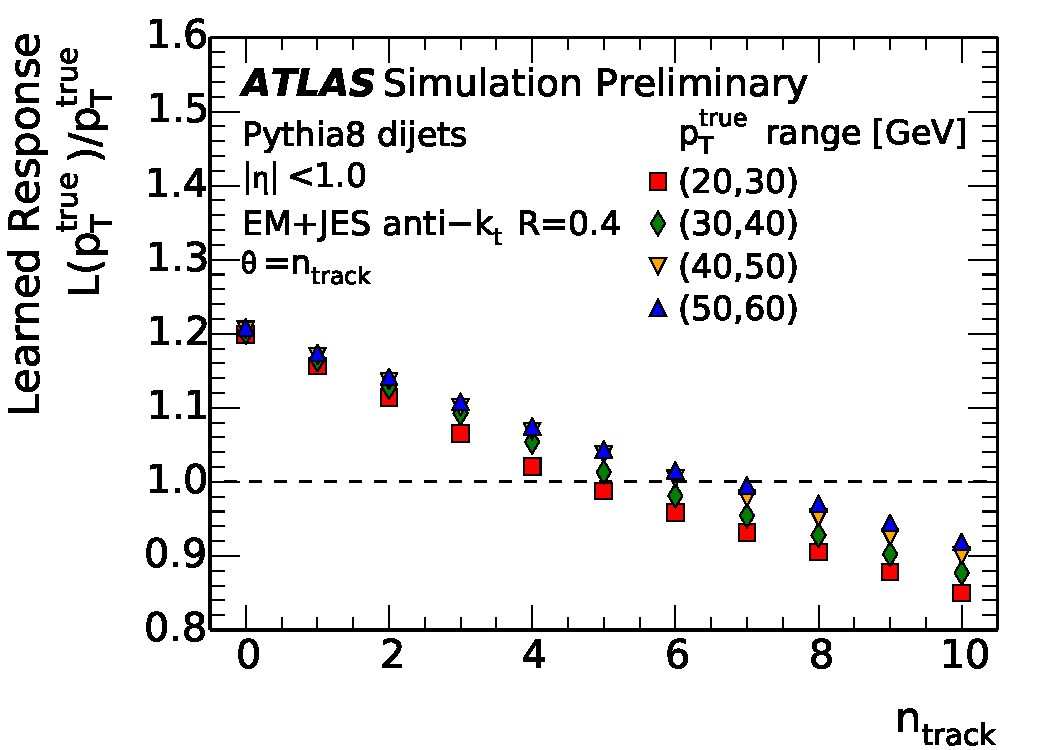
\includegraphics[width=0.33\textwidth]{{figures/ntrack_LR_nTrack_scan_preliminary.pdf}}\label{fig:GenNI:ntrack_wtrackmod_seq_LR_CR_scan:a}}
  \subfloat[]{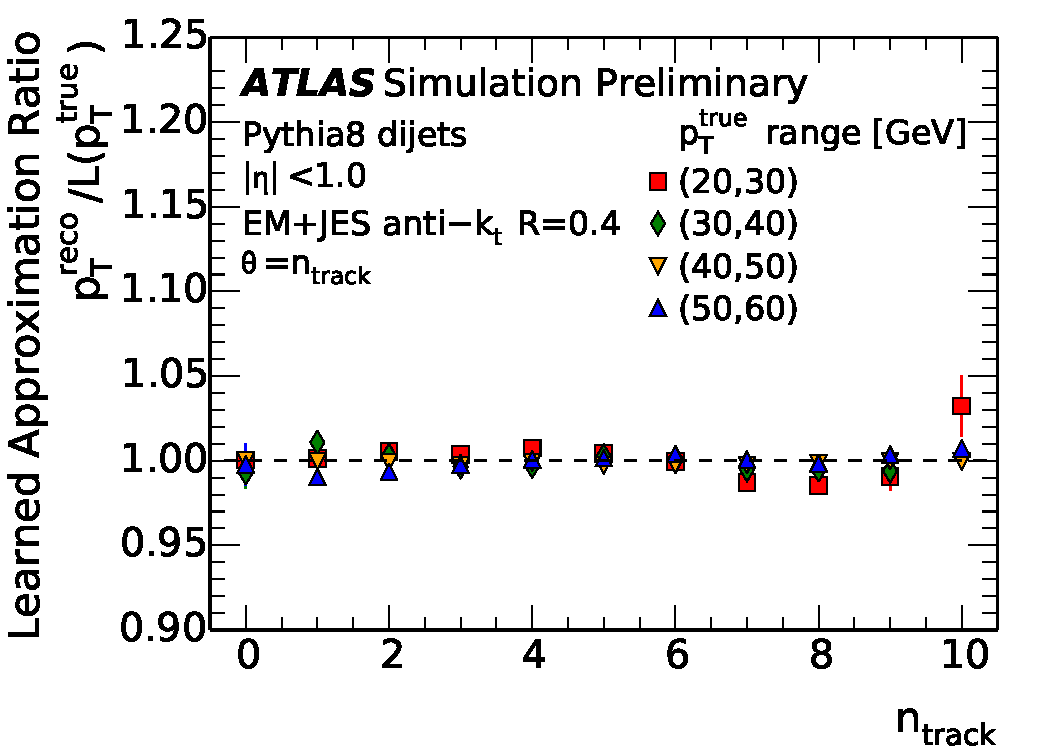
\includegraphics[width=0.33\textwidth]{{figures/ntrack_LR_R_nTrack_scan_preliminary.pdf}}\label{fig:GenNI:ntrack_wtrackmod_seq_LR_CR_scan:b}}
  \subfloat[]{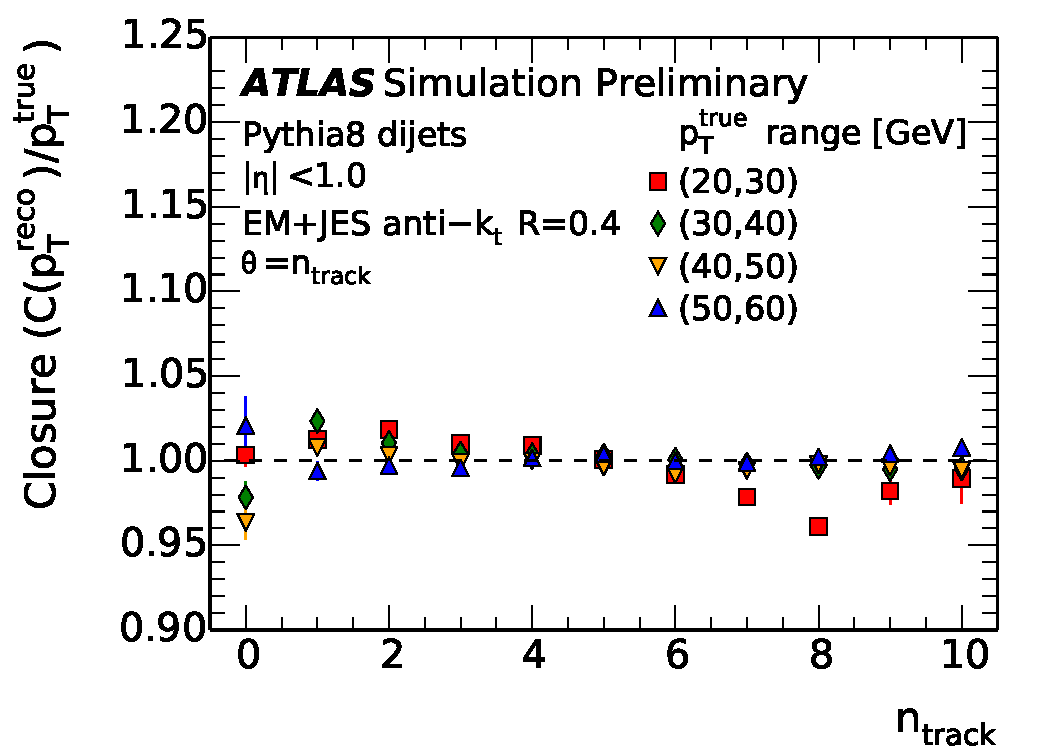
\includegraphics[width=0.33\textwidth]{{figures/ntrack_CR_nTrack_scan_preliminary.pdf}}\label{fig:GenNI:ntrack_wtrackmod_seq_LR_CR_scan:c}}\\
  \subfloat[]{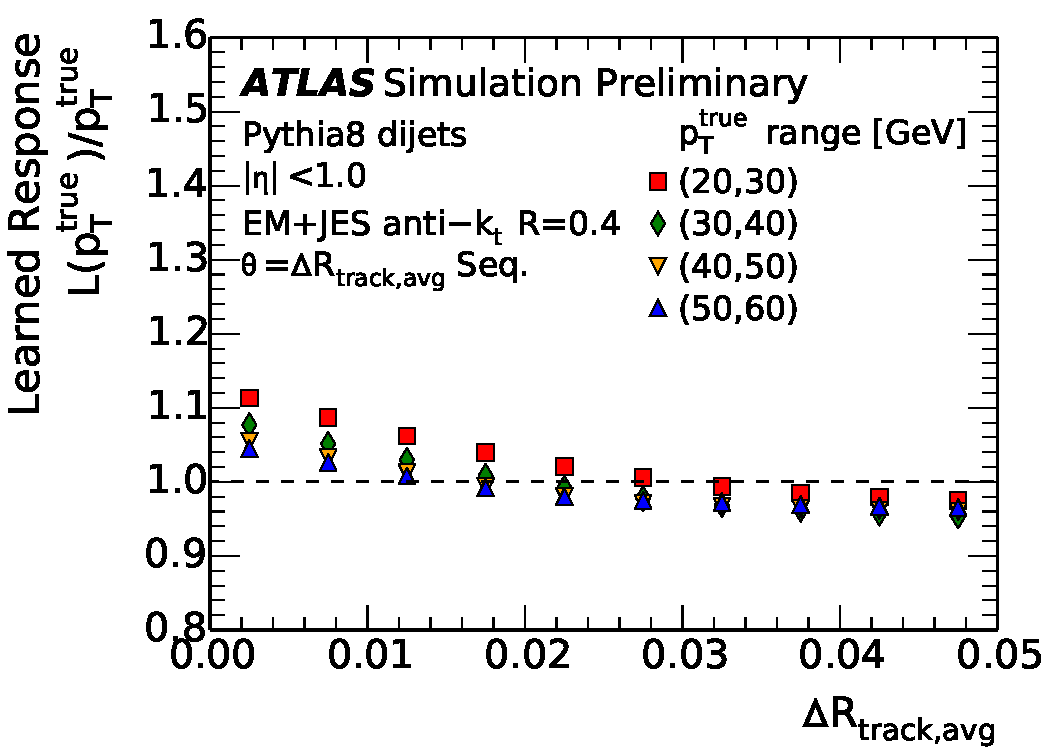
\includegraphics[width=0.33\textwidth]{{figures/ntrack_wtrackmod_seq_LR_wTrack_mod_scan_preliminary.pdf}}\label{fig:GenNI:ntrack_wtrackmod_seq_LR_CR_scan:d}}
  \subfloat[]{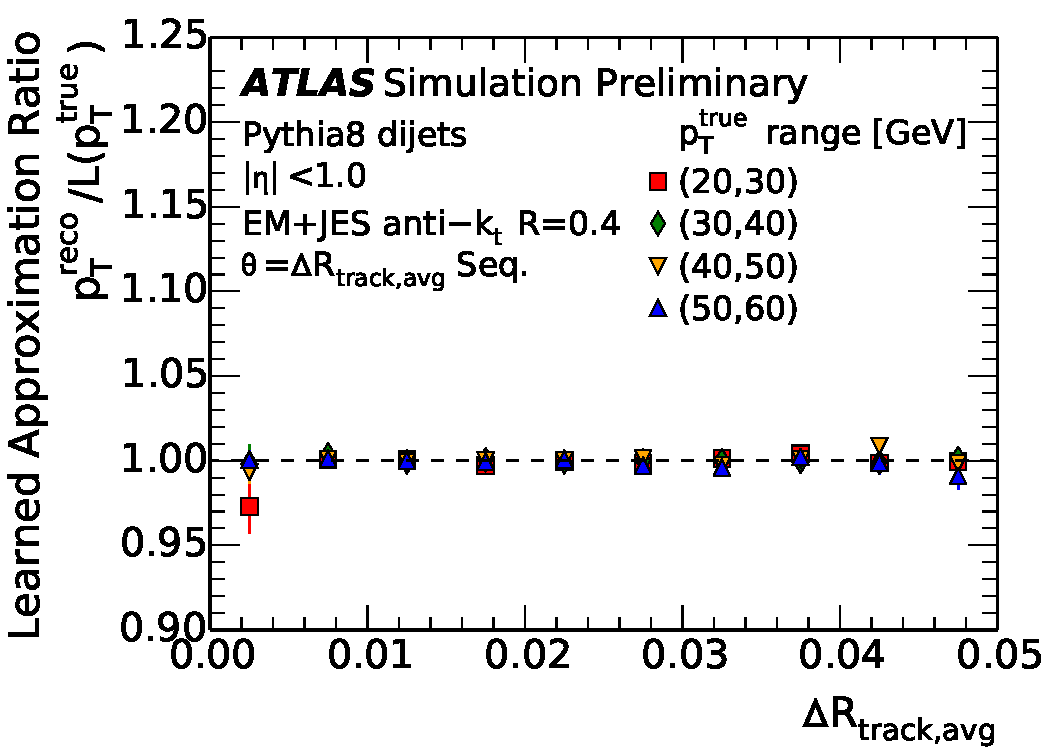
\includegraphics[width=0.33\textwidth]{{figures/ntrack_wtrackmod_seq_LR_R_wTrack_mod_scan_preliminary.pdf}}\label{fig:GenNI:ntrack_wtrackmod_seq_LR_CR_scan:e}}
  \subfloat[]{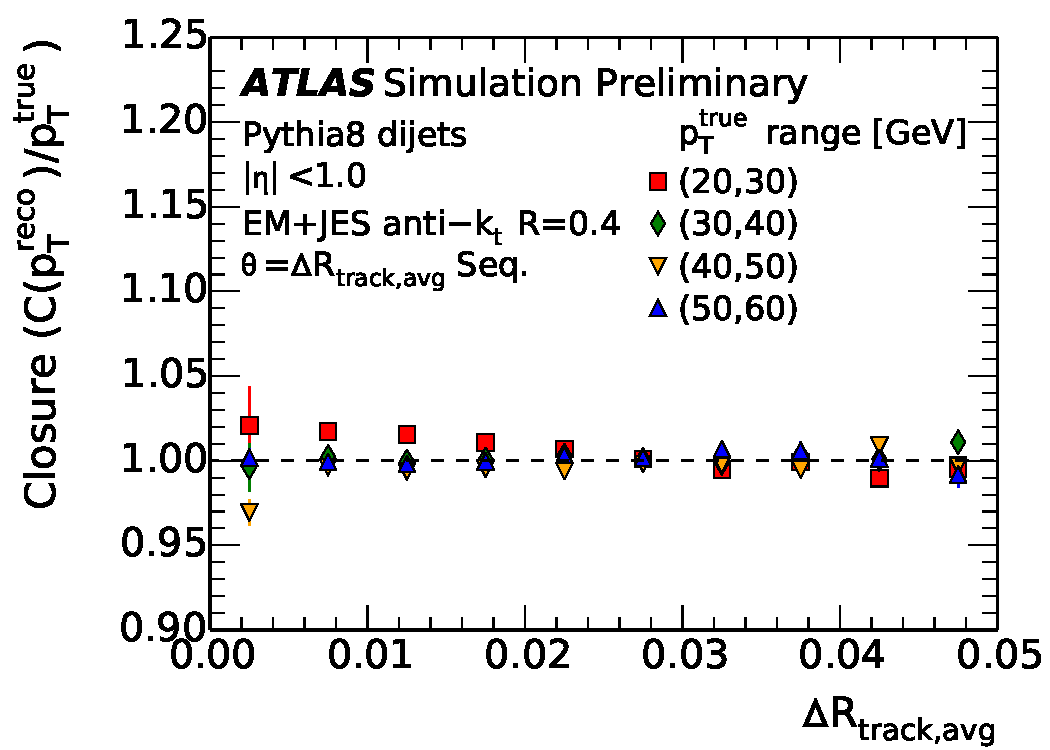
\includegraphics[width=0.33\textwidth]{{figures/ntrack_wtrackmod_seq_CR_wTrack_mod_scan_preliminary.pdf}}\label{fig:GenNI:ntrack_wtrackmod_seq_LR_CR_scan:f}}
  \caption{The dependence of the (a) learned response $L(\pttrue,\theta)/\pttrue$, (b) ratio of $\ptreco$ to learned approximation $L(\pttrue,\theta)$, and (c) calibrated response $C(\ptreco,\theta)/\pttrue$ on $n_\text{track}$ in several bins of truth jet $p_\text{T}$ for $\theta=\{n_\text{track}\}$. Also, the dependence of the (d) learned response $L(\pttrue,\theta)/\pttrue$, (e) ratio of $\ptreco$ to learned approximation $L(\pttrue,\theta)$, and (f) calibrated response $C(\ptreco,\theta)/\pttrue$ on $\Rtrack$ in several bins of truth jet $p_\text{T}$ for $\theta=\{\Rtrack\}$ in sequence after the $n_\text{track}$ correction.
    }
  \label{fig:GenNI:ntrack_wtrackmod_seq_LR_CR_scan}
\end{figure}

Corresponding results for the network trained to simultaneously learn the dependence on $\text{n}_\text{track}$ and $\Rtrack$ are shown in Figure~\ref{fig:GenNI:ntrack_wtrackmod_simul_LR_CR_scan}.
The network is able to learn the dependence on either of the two features in one dimension and Figures~\ref{fig:GenNI:ntrack_wtrackmod_simul_LR_CR_scan:c} and~\ref{fig:GenNI:ntrack_wtrackmod_simul_LR_CR_scan:f} also show that the calibration closes.

\begin{figure}[h!]
  \centering 
  \subfloat[]{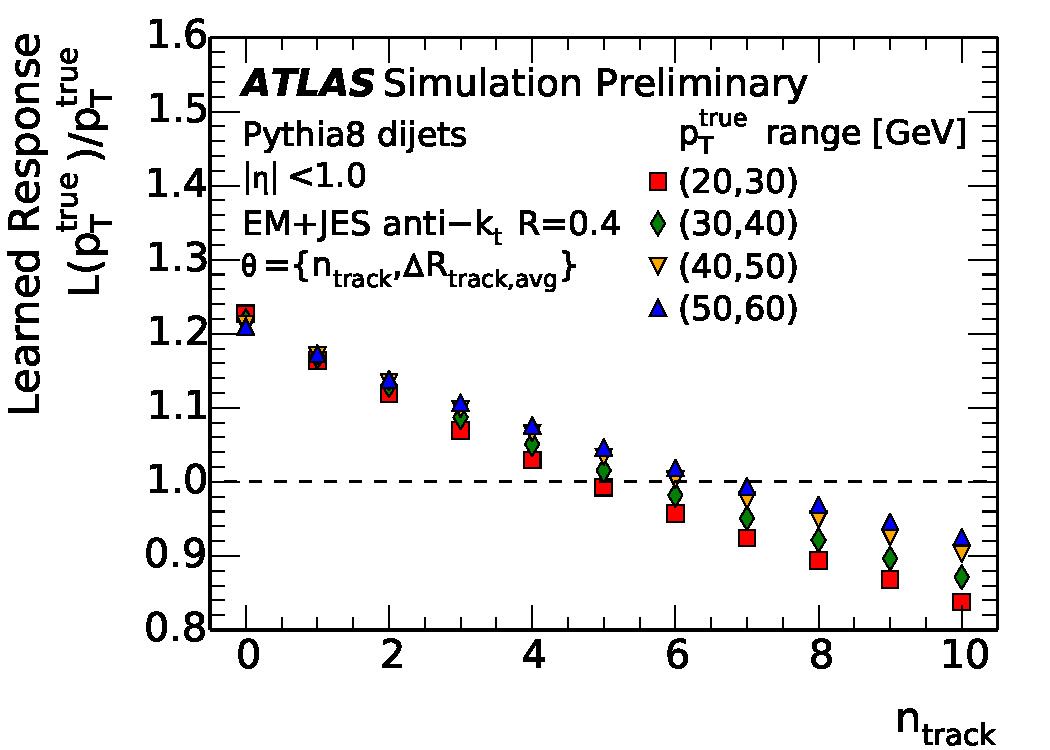
\includegraphics[width=0.33\textwidth]{{figures/ntrack_wtrackmod_simulK3U_LR_nTrack_scan_preliminary.pdf}}\label{fig:GenNI:ntrack_wtrackmod_simul_LR_CR_scan:a}}
  \subfloat[]{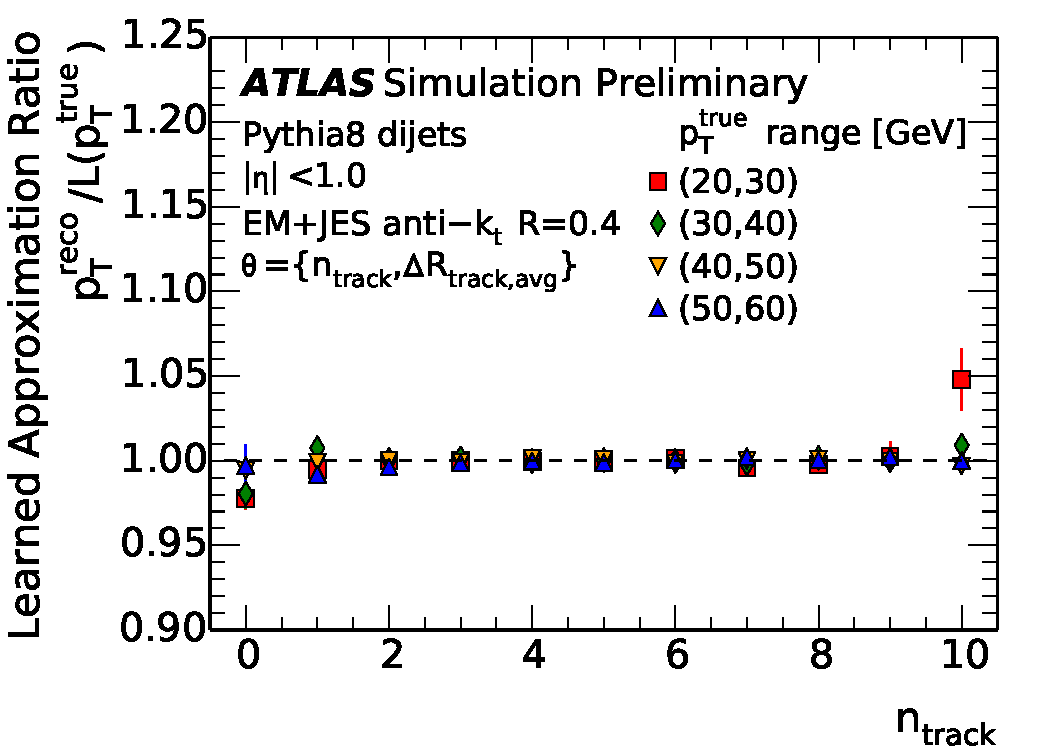
\includegraphics[width=0.33\textwidth]{{figures/ntrack_wtrackmod_simulK3U_LR_R_nTrack_scan_preliminary.pdf}}\label{fig:GenNI:ntrack_wtrackmod_simul_LR_CR_scan:b}}
  \subfloat[]{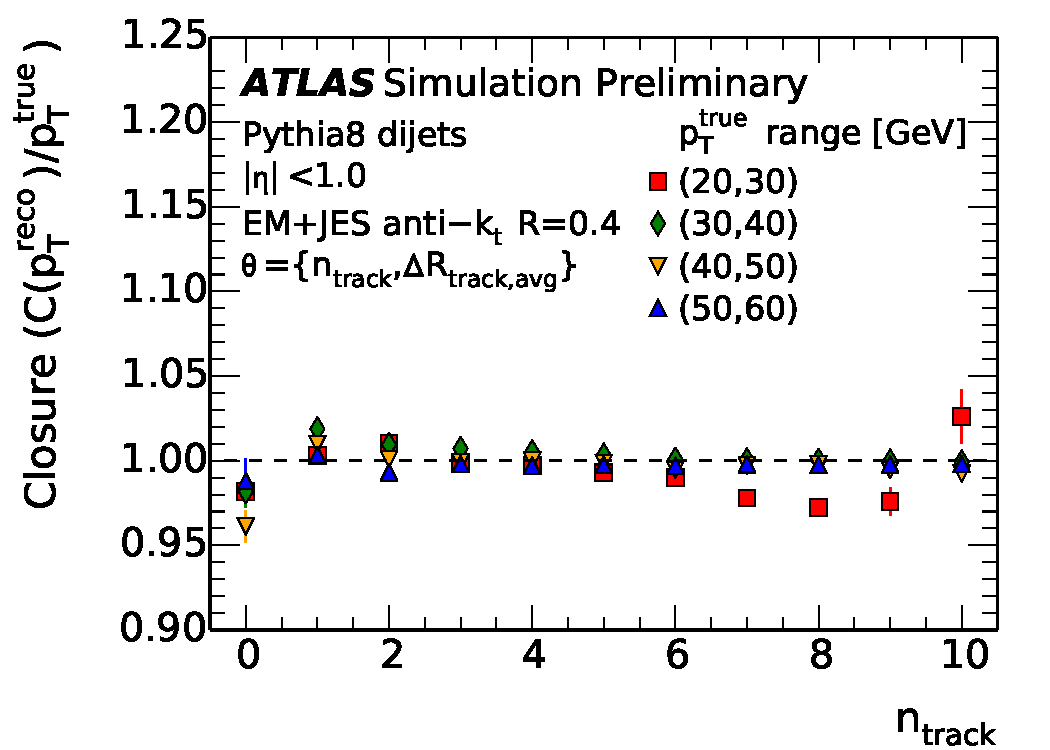
\includegraphics[width=0.33\textwidth]{{figures/ntrack_wtrackmod_simulK3U_CR_nTrack_scan_preliminary.pdf}}\label{fig:GenNI:ntrack_wtrackmod_simul_LR_CR_scan:c}}\\
  \subfloat[]{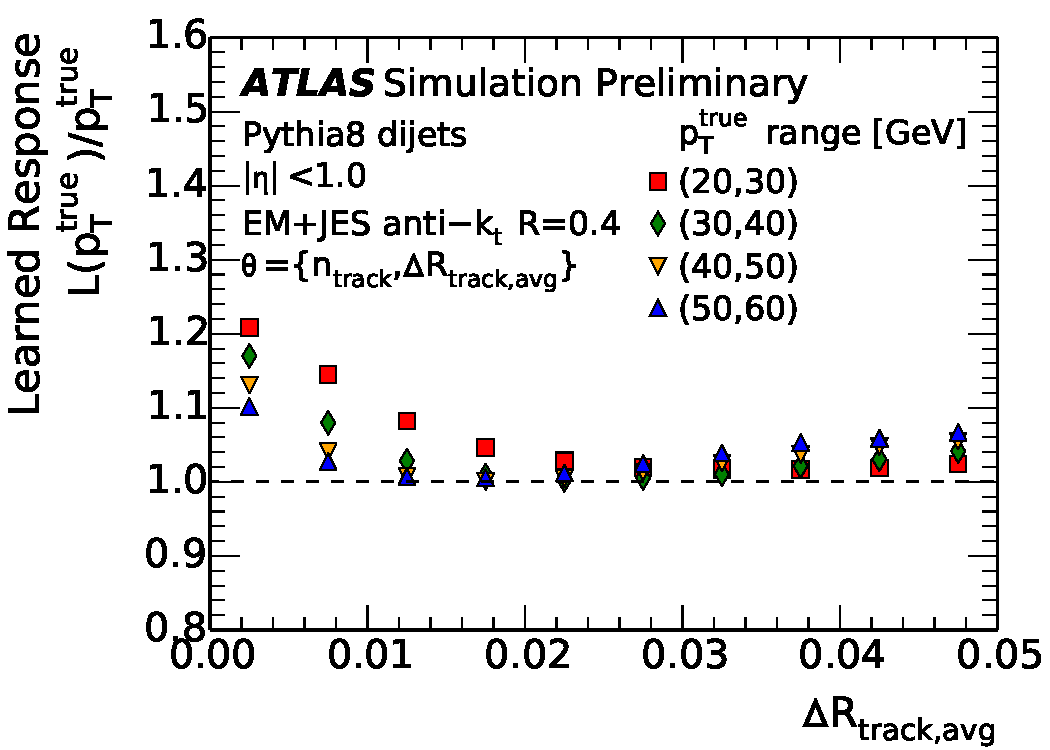
\includegraphics[width=0.33\textwidth]{{figures/ntrack_wtrackmod_simulK3U_LR_wTrack_mod_scan_preliminary.pdf}}\label{fig:GenNI:ntrack_wtrackmod_simul_LR_CR_scan:d}}
  \subfloat[]{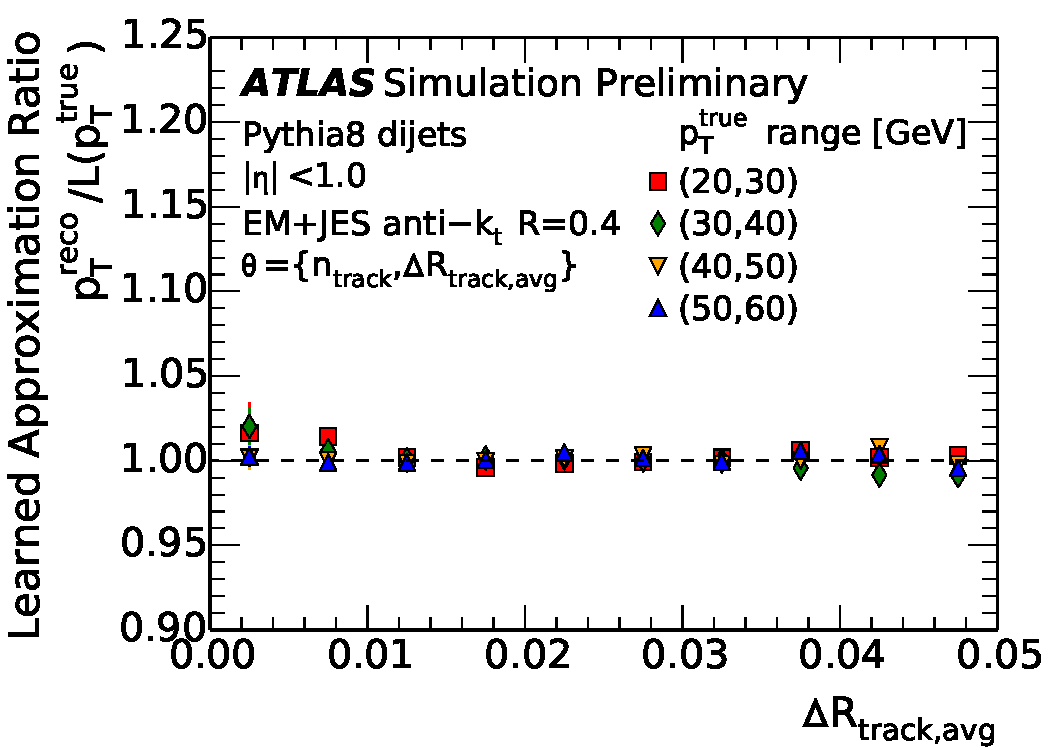
\includegraphics[width=0.33\textwidth]{{figures/ntrack_wtrackmod_simulK3U_LR_R_wTrack_mod_scan_preliminary.pdf}}\label{fig:GenNI:ntrack_wtrackmod_simul_LR_CR_scan:e}}
  \subfloat[]{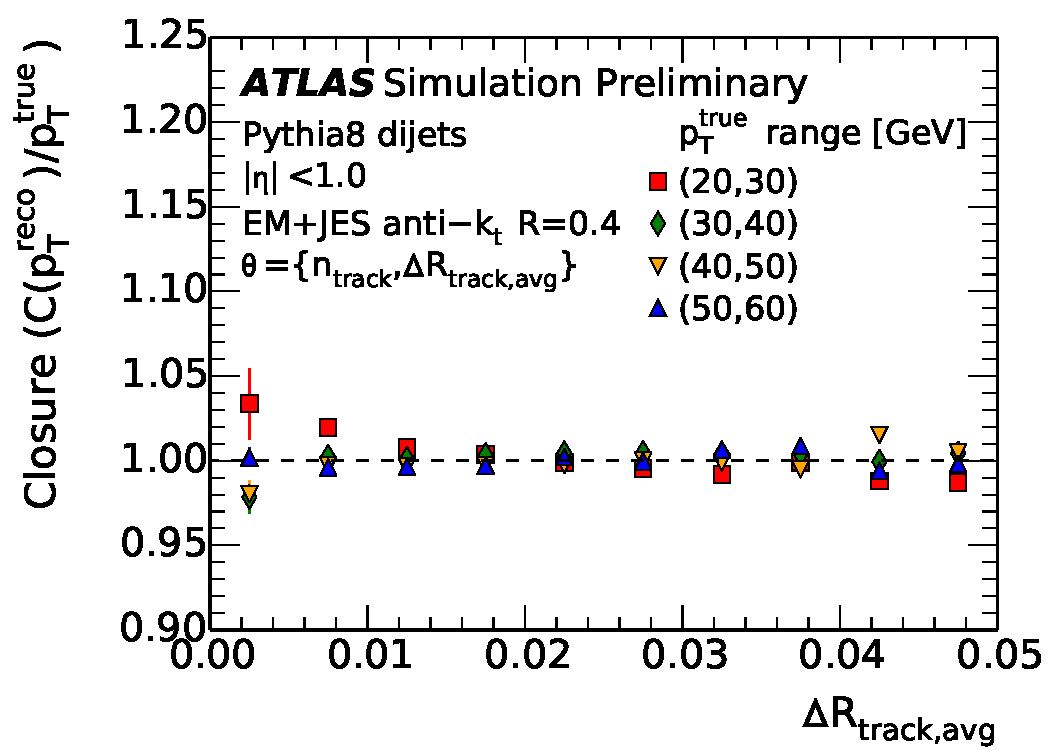
\includegraphics[width=0.33\textwidth]{{figures/ntrack_wtrackmod_simulK3U_CR_wTrack_mod_scan_preliminary.pdf}}\label{fig:GenNI:ntrack_wtrackmod_simul_LR_CR_scan:f}}
  \caption{The dependence of the (a,d) learned response $L(\pttrue,\theta)/\pttrue$, (b,e) ratio of $\ptreco$ to learned approximation $L(\pttrue,\theta)$, and (c,f) calibrated response $C(\ptreco,\theta)/\pttrue$ on (a,b,c) $n_\text{track}$ and (d,e,f) $\Rtrack$, respectively, in several bins of truth jet $p_\text{T}$ for a simultaneous calibration with $\theta=\{n_\text{track},\Rtrack\}$.
    }
  \label{fig:GenNI:ntrack_wtrackmod_simul_LR_CR_scan}
\end{figure}

The advantage of the simultaneous method is highlighted in Figure~\ref{fig:GenNI:dRdntrack_wTrack_mod}.
After the calibration, in each step of the sequential method, there is still a residual dependence of the calibrated response $\hat{R}$ on $\ntrack$ in individual bins of $\Rtrack$.
This residual dependence is monotonic, and so the single value $d\hat{R}/d\ntrack$ (obtained as the slope when fitting $\hat{R}$ versus $\ntrack$ to a line in bins of $\Rtrack$) parameterizes the remaining residual dependence.
The residual dependence on $\ntrack$ in bins of $\Rtrack$ is nearly the same and clearly not zero at all values of $\Rtrack$ if the $\text{n}_\text{track}$ or sequential $\text{n}_\text{track}$, $\Rtrack$ calibrations are applied.
However, the residual dependence is zero and independent of $\Rtrack$ when the simultaneous calibration is performed.
Similarly, there is still a residual dependence of $d\hat{R}/d\Rtrack$ on $\ntrack$ if the $\ntrack$ or sequential $\ntrack$, $\Rtrack$ calibrations are applied; this residual dependence goes away with the simultaneous calibration.

For example, in the sequential calibration, $d\hat{R}/d\ntrack \approx -0.02$ for large $\Rtrack$.
This means that two jets with values of $\ntrack$ differing by $5$ (and the same large values of $\Rtrack$) will have a response difference of $\sim 0.1$.
Similarly, in the sequential calibration, $d\hat{R}/d\Rtrack \approx -4$ for large $\ntrack$.
Two jets that differ in $\Rtrack$ by $0.02$ (both with large $\ntrack$) will therefore have a response difference of $\sim 0.08$.

Because of this residual dependence, there can be nonclosures in specific regions of the parameter space, despite the calibration closing inclusively overall.
Figure~\ref{fig:GenNI:dRdntrack_wTrack_mod:c} shows a selection on $\ntrack$ and $\Rtrack$ which is more efficient on gluons than on quarks, and Figure~\ref{fig:GenNI:dRdntrack_wTrack_mod:d} shows a selection which is more efficient on quarks than on gluons.
In the sequential calibration, large non-closures can be seen in some regions of the parameter space, while the simultaneous calibration almost completely removes these nonclosures.

\begin{figure}[t]
  \centering 
  \subfloat[]{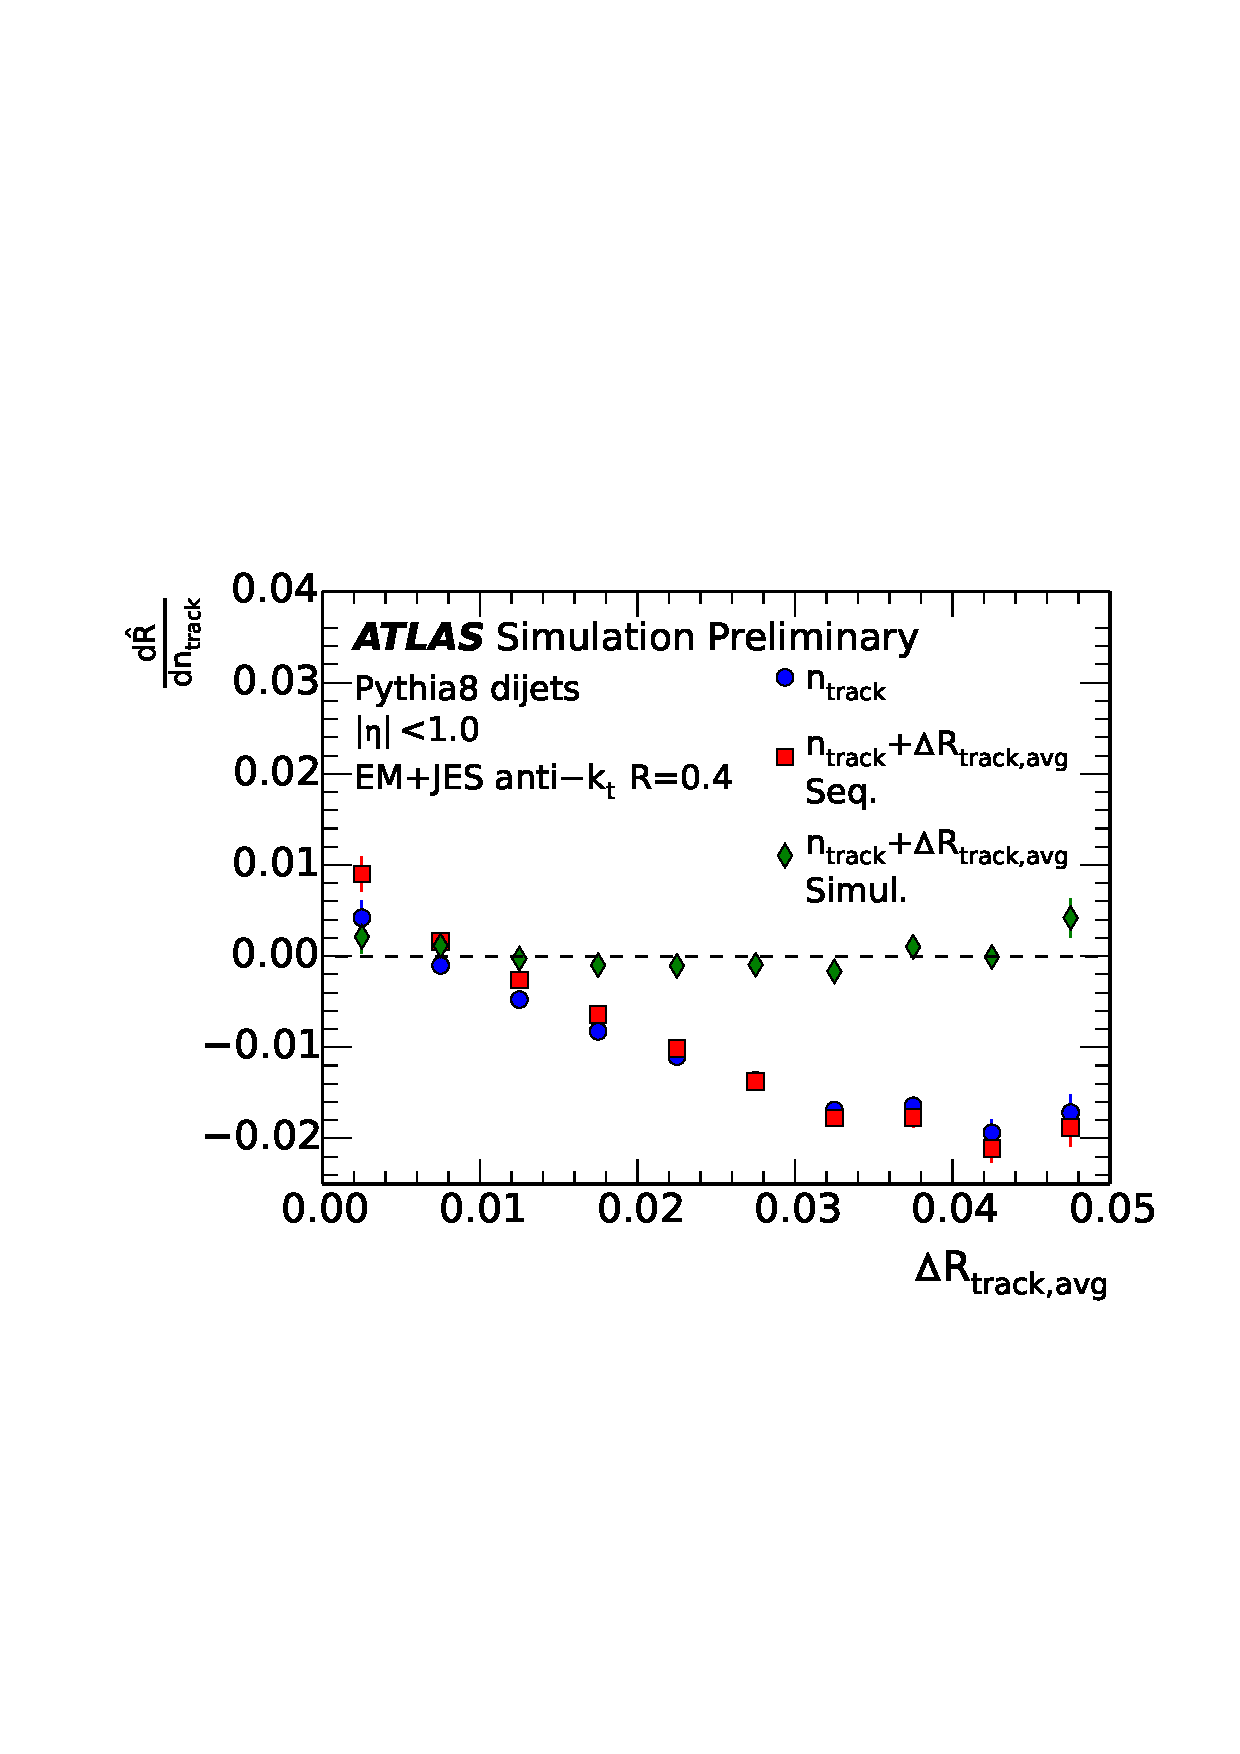
\includegraphics[width=0.45\textwidth]{{figures/dRdntrack_wTrack_mod_ntrack_wtrackmod_preliminary}.pdf}\label{fig:GenNI:dRdntrack_wTrack_mod:a}}
  \subfloat[]{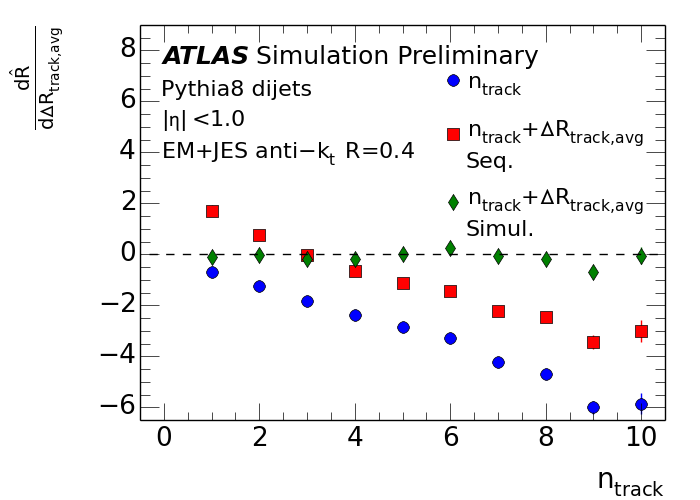
\includegraphics[width=0.45\textwidth]{{figures/dRdwTrack_mod_ntrack_ntrack_wtrackmod_preliminary}.pdf}\label{fig:GenNI:dRdntrack_wTrack_mod:b}}\\
  \subfloat[]{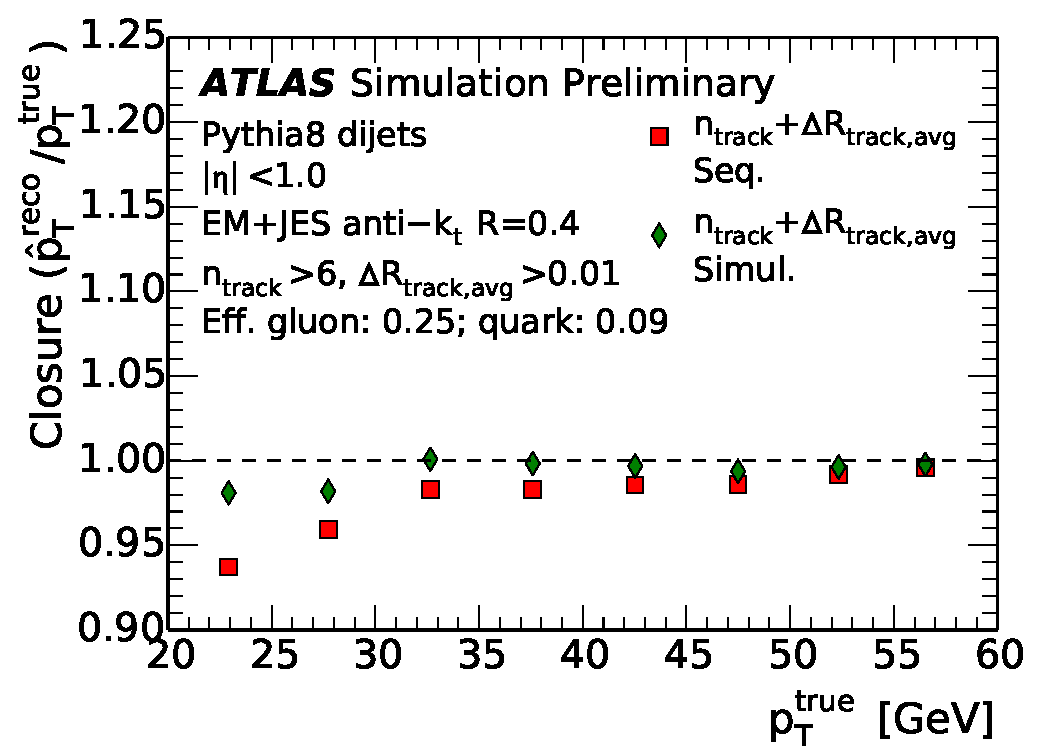
\includegraphics[width=0.45\textwidth]{{figures/CR_x_compare_ntrack_wtrackmod_all_ntrackg6_wtrackmodg010_preliminary}.pdf}\label{fig:GenNI:dRdntrack_wTrack_mod:c}}
  \subfloat[]{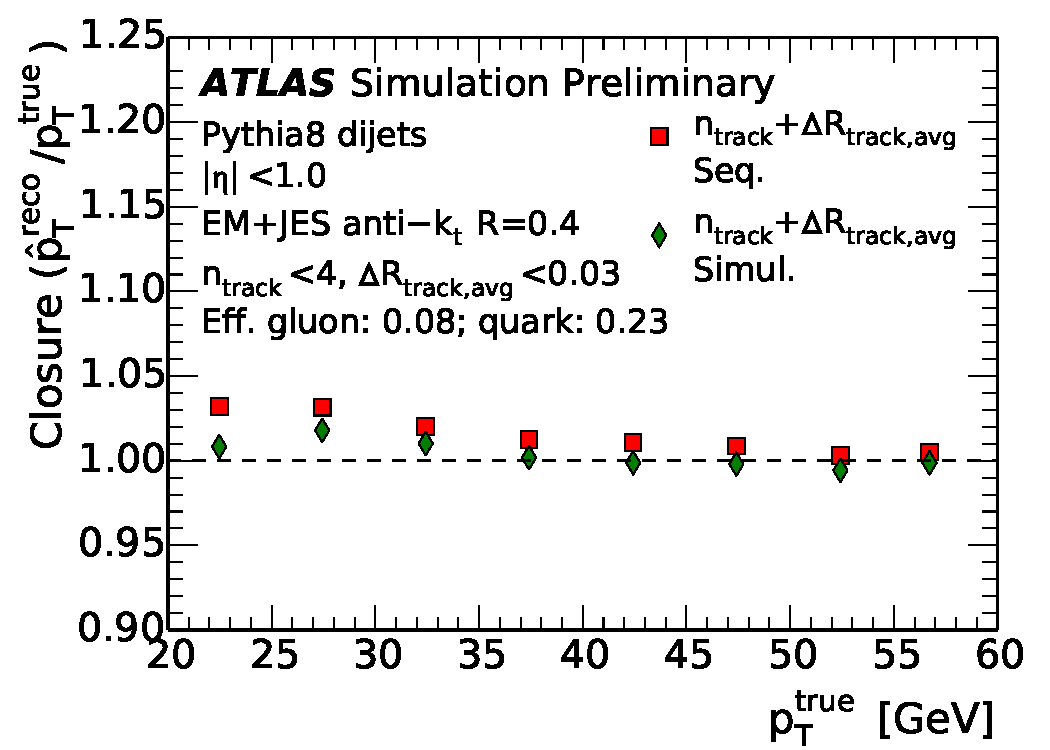
\includegraphics[width=0.45\textwidth]{{figures/CR_x_compare_ntrack_wtrackmod_all_ntrackl4_wtrackmodl030_preliminary}.pdf}\label{fig:GenNI:dRdntrack_wTrack_mod:d}}\\
  \caption{The dependence of (a) $\frac{d\hat{R}}{dn_\text{track}}$ on $\Rtrack$ and (b) $\frac{d\hat{R}}{d\Rtrack}$ on $\ntrack$ for: a calibration using a network with $\theta=\{n_\text{track}\}$ (circles); a calibration using a network with $\theta=\{\Rtrack\}$ employed sequentially after correcting for $n_\text{track}$ (squares); and a simultaneous calibration using a network with $\theta=\{n_\text{track},\Rtrack\}$ (diamonds).
    Also, the closure as a function of $\pttrue$, in (c) a selection intended to target gluon jets; and (d) a selection intended to target quark jets.
    }
  \label{fig:GenNI:dRdntrack_wTrack_mod}
\end{figure}

As observables correlated with the quark or gluon provenance of a jet, the correction for the dependence of the energy on $\text{n}_\text{track}$ and $\Rtrack$ can reduce the response difference between jet types.
Figure~\ref{fig:GenNI:quarkgluon_wtrackmod} shows the difference between the  response for quark and gluon jets as a function of the truth jet $p_\text{T}$ for different calibration methods.
Since gluon jets have a softer constituent $p_\text{T}$ spectrum, their response is lower than for quark jets on average.
The residual correction does reduce the response difference; the simultaneous approach is slightly better than the sequential approach at every value of truth jet $p_\text{T}$.

The properties of quark and gluon jets can depend on the specific model of jet fragmentation used; therefore, it is also important to check that the improvement in the quark-gluon response difference is robust to these model differences.
In addition to showing the results for \PYTHIA~8, Figure~\ref{fig:GenNI:quarkgluon_wtrackmod:b} also demonstrates that (without retraining) there are also improvements for \textsc{Herwig}~7. 

\begin{figure}[h!]
  \centering 
  \subfloat[ \PYTHIA~8]{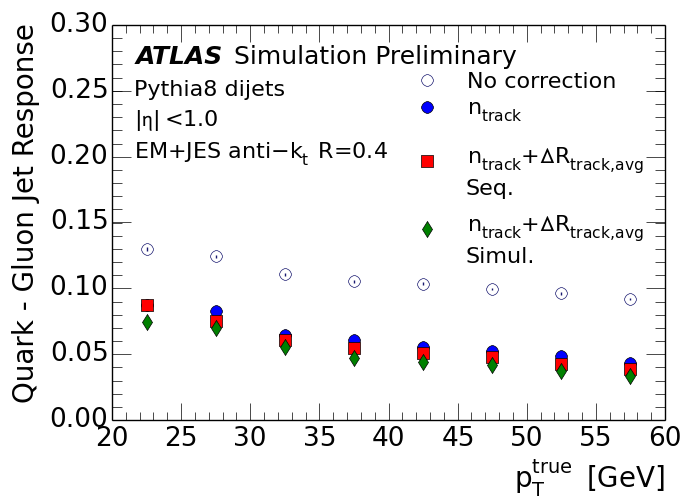
\includegraphics[width=0.45\textwidth]{{figures/quarkgluon_JZ3_Pythia_wtrackmod_ntrack_preliminary}.pdf}\label{fig:GenNI:quarkgluon_wtrackmod:a}}
  \subfloat[\textsc{Herwig}~7 ]{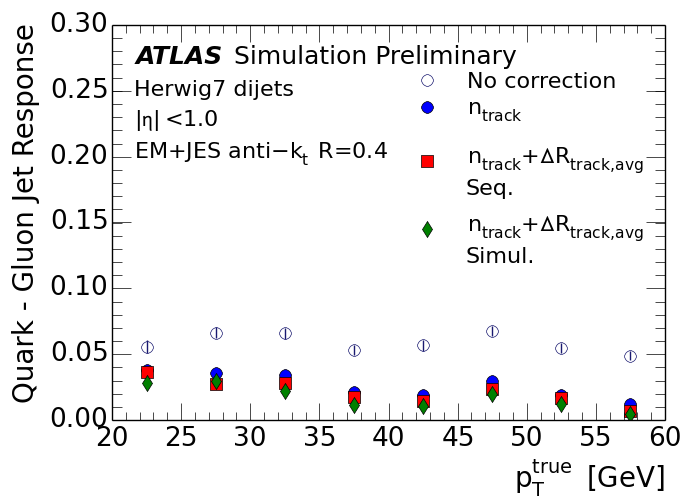
\includegraphics[width=0.45\textwidth]{{figures/quarkgluon_JZ3_Herwig_wtrackmod_ntrack_preliminary}.pdf}\label{fig:GenNI:quarkgluon_wtrackmod:b}}
  \caption{The difference between the response of quarks and gluons as a function of $\pttrue$ for: before any $n_\text{track}$ or $\Rtrack$ correction (open circles); a calibration using a network with $\theta=\{n_\text{track}\}$ (circles); a calibration using a network with  $\theta=\{\Rtrack\}$ sequentially after correcting for $n_\text{track}$ (squares); and a simultaneous calibration using a network with $\theta=\{n_\text{track},\Rtrack\}$ (diamonds).
    }
  \label{fig:GenNI:quarkgluon_wtrackmod}
\end{figure}


%It is also interesting to study the residual response dependence on $\text{n}_\text{track}$ and $\Rtrack$ for a given parton type.  This will show the impact of the calibration on reducing the sensitivity (and thus the systematic uncertainty) of the modeling of jet fragmentation.   Figure~\ref{fig:GenNI:nonclosure_ntrack_quarkgluon} shows the non-closure as a function of $n_\text{track}$ for quark and gluon jets separately, after a sequential or simultaneous calibration.  For quark jets ((c) and (d) of Fig.~\ref{fig:GenNI:nonclosure_ntrack_quarkgluon}) there is a clear reduction in the non-closure from the simultaneous (d) over the sequential calibration (c).   Especially at low $p_\text{T}$, this reduction can reach 20\%.  For gluon jets ((a) and (b)), there is a reduction at high $n_\text{track}$, but not at low $n_\text{track}$.

Another goal of the correction based on auxiliary variables is to reduce the sensitivity of the jet energy to mismodeling of the underlying features.
An important consequence of such a reduction could be a smaller systematic uncertainty associated with jet fragmentation modeling.
Figure~\ref{fig:GenNI:respdiff_PythiaHerwig} quantifies this effect by showing the difference in the jet response between \PYTHIA~8 and \textsc{Herwig}~7 for quarks and gluons separately.
It can be seen that the jet response difference between the generators is generally better in the simultaneous calibration method than in the sequential method. 
In particular, in some bins of $\pttrue$, the sequential method makes the difference between the generators worse than not including the second variable, while the simultaneous method retains or slightly improves the difference between the generators.
This could happen if the correlation between the two features changes between the generators in such a way that the sequential calibration effectively undoes the correction of the first feature in the sample the network was not trained on.
Another possible effect is that the correlation between the two features stays the same between the generators, but the underlying distribution of one or both of the features in the jets changes.
In either case, since the simultaneous method conditions on both features at once, this does not affect the final performance.

\begin{figure}[h!]
  \centering 
  \subfloat[]{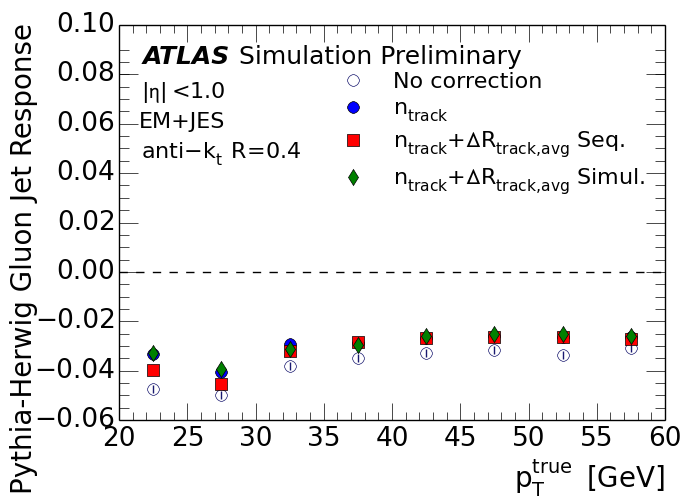
\includegraphics[width=0.45\textwidth]{{figures/PythiaHerwig_JZ3_gluon_wtrackmod_ntrack_preliminary}.pdf}}
  \subfloat[]{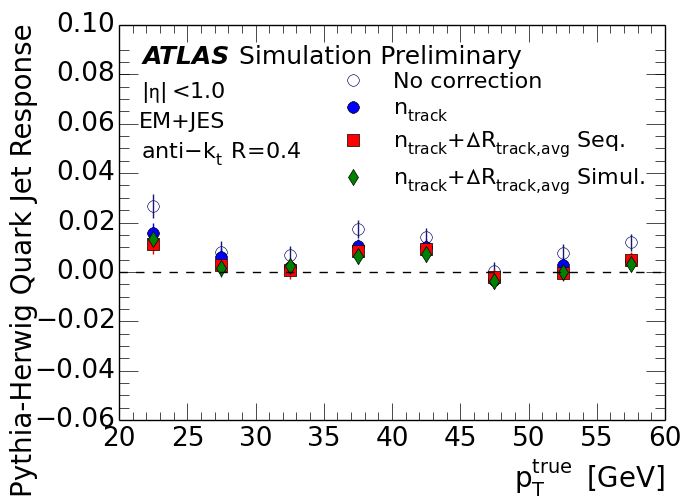
\includegraphics[width=0.45\textwidth]{{figures/PythiaHerwig_JZ3_quark_wtrackmod_ntrack_preliminary}.pdf}}
  \caption{The difference between the response of jets in Pythia8 and Herwig7 as a function of $\pttrue$ in (a) gluon jets, and (b) quark jets, for: before any $n_\text{track}$ or $ \Rtrack$ correction (open circles); a calibration using a network with $\theta=\{n_\text{track}\}$ (circles); a calibration using a network with  $\theta=\{ \Rtrack\}$ sequentially after correcting for $n_\text{track}$ (squares); and a simultaneous calibration using a network with $\theta=\{n_\text{track}, \Rtrack\}$ (diamonds).
    }
  \label{fig:GenNI:respdiff_PythiaHerwig}
\end{figure}


A final metric for studying the impact of generalized numerical inversion is the jet energy resolution.
One component of the jet energy resolution is due to the spread in the jet energy response for various values of $\theta$ - in the extreme case that there is no spread in $p_\text{T}^\text{reco}$ given $p_\text{T}^\text{true}$ and $\theta$, there will still be an effective resolution resulting from the spread in values over the range of $\theta$.
However, as mentioned in Section~\ref{sec:GenNI:jetreco} and expounded upon in Appendix~\ref{sec:GenNI_app:auxiliary}, the calibrated resolution does not necessarily improve following the correction based on auxiliary variables.
Figure~\ref{fig:GenNI:stdCR_x_compare_ntrack_wtrackmod} shows both the inclusive (not differential in $\theta$) closure as well as the inclusive resolution as a function of the truth jet $p_\text{T}$, for different calibration methods.
All methods achieve a similar inclusive closure and as desired, the residual calibration procedures reduce the resolution.
The overall resolution reduction is similar for the sequential and simultaneous approaches, with the simultaneous slightly better at higher $p_\text{T}$ and the sequential slightly better at low $p_\text{T}$.
The difference in the resolutions from the various approaches is small compared to the gain over no residual calibration.

%\begin{figure}[t]
%  \centering 
%  \subfloat[]{\includegraphics[width=0.45\textwidth]{{dRdnTrack_quark_ntrack_wtrackmod_seq}.png}}
%  \subfloat[]{\includegraphics[width=0.45\textwidth]{{dRdnTrack_quark_ntrack_wtrackmod_simulK3U}.png}}
%  \caption{A caption.
%    }
%  \label{fig:GenNI:dRdnTrack_quark_ntrack_wtrackmod_seq}
%\end{figure}

\begin{figure}[t]
  \centering 
  \subfloat[]{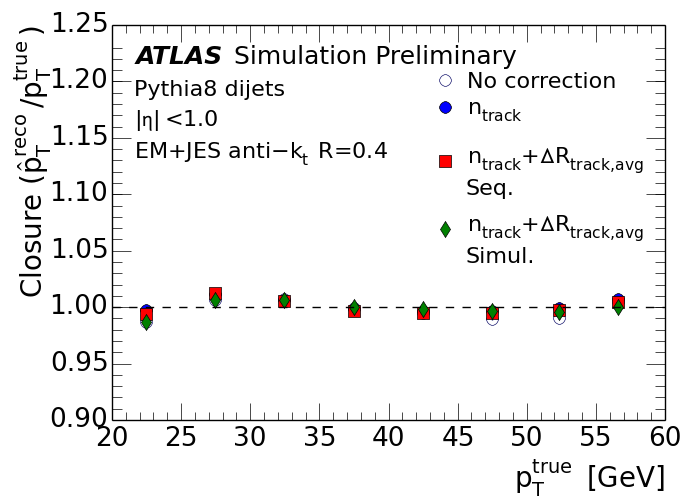
\includegraphics[width=0.45\textwidth]{{figures/CR_x_compare_ntrack_wtrackmod_all_preliminary}.pdf}}
  \subfloat[]{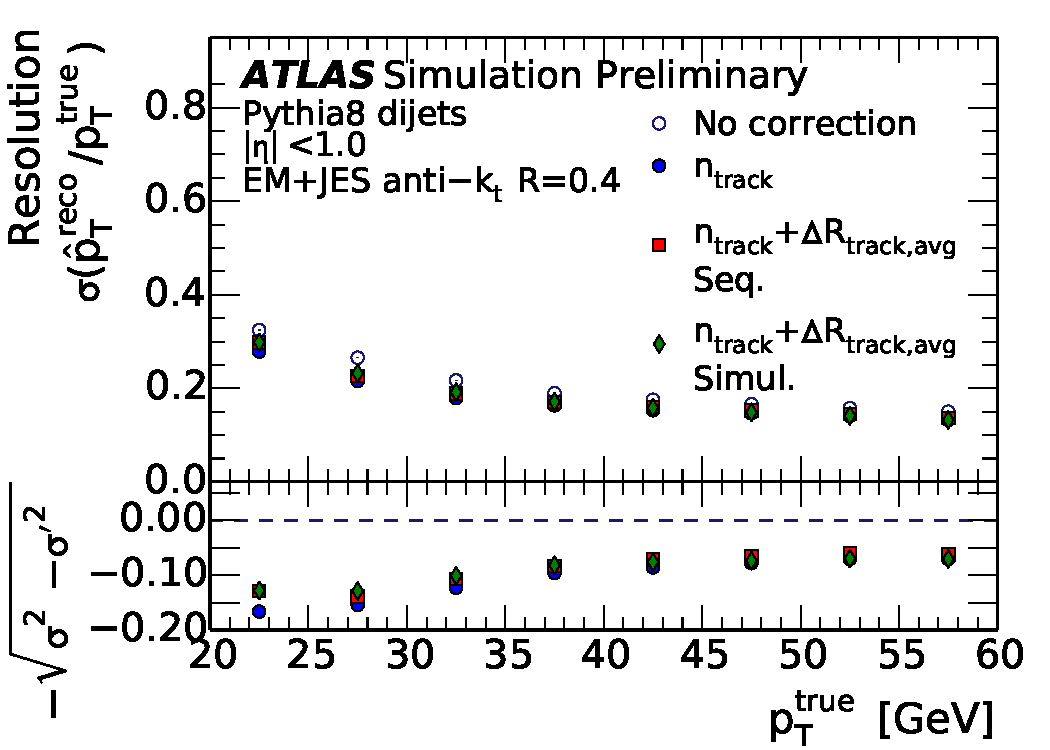
\includegraphics[width=0.45\textwidth]{{figures/stdCR_x_compare_ntrack_wtrackmod_all_preliminary}.pdf}}
  \caption{The (a) closure and (b) resolution as a function of $\pttrue$ for: before any $n_\text{track}$ or $\Rtrack$ correction (open circles); a calibration using a network with $\theta=\{n_\text{track}\}$ (circles); a calibration using a network with  $\theta=\{\Rtrack\}$ sequentially after correcting for $n_\text{track}$ (squares); and a simultaneous calibration using a network with $\theta=\{n_\text{track},\Rtrack\}$ (diamonds).
    For the resolution, also shown is the (negative) improvement in quadrature of the resolution for a given calibration with resolution $\sigma^\prime$ to the resolution before any correction $\sigma$.
  }
  \label{fig:GenNI:stdCR_x_compare_ntrack_wtrackmod}
\end{figure}

% All figures and tables should appear before the summary and conclusion.
% The package placeins provides the macro \FloatBarrier to achieve this.
%\FloatBarrier

\FloatBarrier

%-------------------------------------------------------------------------------
\section{Discussion}
\label{sec:GenNI:discussion}
%-------------------------------------------------------------------------------
The results presented in Section~\ref{sec:GenNI:results} demonstrate that the simultaneous neural network-based method introduced in this Chapter improves the performance of the calibration on a variety of metrics.
%In addition to directly removing the dependence of the energy on the features and combinations of the features themselves, Section~\ref{sec:GenNI:intro} outlined three metrics by which the correction based on auxiliary variables may improve the calibration: reducing the difference between quark and gluon jets, reducing the effect of mismodeling the underlying features, and improving the inclusive resolution.

The search in Chapter~\ref{ch:HBSM} involves both quarks and gluons in the final state, and tagging the jets~\cite{ATL-PHYS-PUB-2017-009,Aad:2014gea,ATLAS-CONF-2016-034,ATL-PHYS-PUB-2017-017} may help both with background reduction and with the combinatorial problem of determining the jets decaying from the $a$ particle and the ones associated with the VBF production.
Figures~\ref{fig:GenNI:dRdntrack_wTrack_mod:c} and~\ref{fig:GenNI:dRdntrack_wTrack_mod:d} show directly the reductions of non-closures when using the simultaneous method in selections targeting gluons and quarks, respectively.
Any nonclosures can reduce the sensitivity of the analysis, in particular in the gluon jets, as the resolution of the $m_{jj}$ derived from the gluon jets is a major limitation in the analysis.

In addition, if there is a dependence of the energy response on the underlying features then any mismodeling in the distribution of those features can affect the final energy and introduce systematic uncertainties.
The low-mass extension of this search discussed in Appendix~\ref{sec:HBSM_app:lowmass} proposes in particular the use of small-$R$ jet substructure to tag the boosted low-mass decays, and so therefore reducing any uncertainties associated with that kind of selection can improve the optimality and sensitivity of the analysis.

The search in Chapter~\ref{ch:CWoLa} uses only large-$R$ jets, which as mentioned in Section~\ref{sec:GenNI:jetreco} do not have any GSC applied.
However, large-$R$ jets actually have two relevant parameters with dimensions of energy associated with them - their energy and their mass.
The large-$R$ calibration calibrates the energy first and then the mass in sequence, taking into account the energy as a feature.
Generalized numerical inversion can apply directly to this second step of the large-$R$ jet calibration in order to improve the mass scale - as this search tags on the masses of the involved large-$R$ jets, any improvement on the mass scale directly improves the tagging capabilities and performance of the search.

The technique outlined here does not address the question of how to simultaneously calibrate multiple features, e.g. the jet energy and mass at the same time.
The Author has contributed to a project~\cite{ATL-PHYS-PUB-2020-001} in which an extension of generalized numerical inversion is proposed that addresses exactly this question, and it is found that it is possible to calibrate multiple variables simultaneously while taking into account multiple simultaneous auxiliary variables.
In particular, this project answers this question in the context of the large-$R$ jet calibration, which could directly further improve the sensitivity of the search in Chapter~\ref{ch:CWoLa}.

One point that is not addressed in the formulation of generalized numerical inversion is the difference between the mean, median, and mode of the target distributions; this difference was expounded on particularly thorougly in the discussion of numerical inversion itself in Chapter~\ref{ch:NI}.
The neural network $L$ in generalized numerical inversion learns whatever the loss function indicates it to learn; e.g., if the loss is a mean squared loss then it learns the mean over the corresponding distribution.
The Author has contributed to a project~\cite{Cheong:2019upg} which discusses exactly how to learn the mean, median, or mode of the corresponding distributions with neural networks.
This technique can be used to more closely align with the physics goals of the ATLAS jet calibration.

%-------------------------------------------------------------------------------
\section{Conclusion}
\label{sec:GenNI:conclusion}
%-------------------------------------------------------------------------------

%This chapter has presented a study of a regression-based residual jet energy calibration procedure, implemented with neural networks and designed to avoid binning effects and incorporate correlations in the response between various jet features.  This new method can eliminate the residual dependence on one feature after calibrating for a second feature with a strong influence on the response for the first feature.  This can be useful for mitigating the response difference between quark and gluon jets as well as for reducing the residual dependence on the feature for quark or gluon jets separately.  The simultaneous calibration offers similar benefits to the sequential calibration for the jet energy resolution and by construction has no impact on the inclusive closure of the jet calibration.  Generalized numerical inversion is a promising method for the future as more information about jets is included in the calibration procedure.  Further studies are required to incorporate more observables and quantify the potential reduction in the topology dependence and systematic uncertainties of the full approach.

This Chapter has presented a novel regression-based jet energy calibration procedure implemented with neural networks, called generalized numerical inversion.
Generalized numerical inversion generalizes numerical inversion and in particular retains the key property of being independent of the underlying spectrum (Chapter~\ref{ch:NI}).
The new method is able to take into account multiple auxiliary jet features simultaneously, which is an improvement over the current sequential method - in particular, correlations in the response between various jet features can be corrected for.
The new technique is shown to reduce the response difference between quark and gluon jets by using features associated with the jet provenance, and furthermore is shown to mitigate the effect of mismodeling of the underlying disrtribution of the features themselves.
The simultaneous calibration offers similar benefits to the sequential calibration for the jet energy resolution and by construction has no impact on the inclusive closure of the jet calibration.
These improvements and new extensions of this technique can directly improve the performance of the searches presented in this Thesis (Chapter~\ref{ch:HBSM} and Chapter~\ref{ch:CWoLa}) and of searches and measurements in ATLAS in general.
